% ============================================================
% Main document — PFE Thesis
% ============================================================
\documentclass[12pt,a4paper]{report}
% ============================================================
% Preamble — Shared packages, settings, and custom commands
% ============================================================

% ── Language & encoding ─────────────────────────────────────
\usepackage{fontspec}
\usepackage{polyglossia}
\setmainlanguage{english}
\setotherlanguage{arabic}
\newfontfamily\arabicfont[Script=Arabic,Scale=1.15]{Arabic Typesetting}
\providecommand{\UseMathForPositioningText}{}
\setmainfont{Latin Modern Roman}
\usepackage{csquotes}

% ── Page geometry ───────────────────────────────────────────
\usepackage[a4paper, top=2.5cm, left=2.5cm, right=2.5cm, bottom=2.5cm, footskip=1cm]{geometry}

% ── Typography ──────────────────────────────────────────────
\usepackage{setspace}
\onehalfspacing
\usepackage{microtype}


% ── Mathematics ─────────────────────────────────────────────
\usepackage{amsmath,amssymb,amsfonts}
\usepackage{mathtools}
\usepackage{bm}

% ── Graphics & figures ──────────────────────────────────────
\usepackage{graphicx}
\graphicspath{{figures/}}
\usepackage{subcaption}
\usepackage{tikz}
\usetikzlibrary{arrows.meta, positioning, shapes.geometric, fit, backgrounds, calc}
\usepackage[edges]{forest}
\usepackage{pgfplots}
\pgfplotsset{compat=1.18}
\usepackage{enumitem}

% ── Tables ──────────────────────────────────────────────────
\usepackage{booktabs}
\usepackage{array}
\usepackage{longtable}
\usepackage{multirow}
\usepackage{chngcntr}              % For changing counter behavior
\usepackage{float}                 % For [H] exact figure placement
\counterwithout{figure}{chapter}   % Continuous figure numbering
\counterwithout{table}{chapter}    % Continuous table numbering
\usepackage{tabularx}              % Auto-width table columns


% ── Colors ──────────────────────────────────────────────────
\usepackage{xcolor}
\definecolor{linkcolor}{RGB}{0,51,102}

% ── Hyperlinks ──────────────────────────────────────────────
\usepackage{hyperref}
\hypersetup{
    colorlinks=true,
    linkcolor=black,
    citecolor=blue,
    urlcolor=blue,
    pdftitle={Prediction of Faults in Photovoltaic Systems Using AI},
    pdfauthor={GUERRAICHE Ahmed Amine, MENASSEL Rayane Ibrahim}
}

% ── Headers & footers ───────────────────────────────────────
\usepackage{fancyhdr}
\fancypagestyle{plain}{
    \fancyhf{}
    \fancyfoot[R]{\thepage}
    \renewcommand{\headrulewidth}{0pt}
    \renewcommand{\footrulewidth}{0pt}
}
\pagestyle{plain}

% ── Captions ────────────────────────────────────────────────
\usepackage[font={small,it},labelfont=bf]{caption}
\captionsetup[figure]{font={small,it},labelfont=bf}
\captionsetup[table]{font={small,it},labelfont=bf}

% ── Bibliography ────────────────────────────────────────────
\usepackage[round]{natbib}         % APA-style author-year citations

% ── Algorithms & code ───────────────────────────────────────
\usepackage{algorithm}
\usepackage{algpseudocode}
\usepackage{listings}
\lstset{
    basicstyle=\ttfamily\small,
    breaklines=true,
    frame=single,
    numbers=left,
    numberstyle=\tiny,
    xleftmargin=2em,
    framexleftmargin=1.5em
}

% ── Cross-referencing ───────────────────────────────────────
\usepackage[capitalise,noabbrev]{cleveref}

% ── Appendices ──────────────────────────────────────────────
\usepackage[toc,page]{appendix}

% ── Custom commands ─────────────────────────────────────────
\newcommand{\R}{\mathbb{R}}
\newcommand{\N}{\mathbb{N}}
\newcommand{\Z}{\mathbb{Z}}
\newcommand{\todo}[1]{\textcolor{red}{\textbf{[TODO: #1]}}}
\newcommand{\note}[1]{\textcolor{blue}{\textbf{[Note: #1]}}}

% ── Metadata ────────────────────────────────────────────────
\title{Prediction of Faults in Photovoltaic Systems from Electrical and Meteorological Data Using Artificial Intelligence and Deployment on Jetson Nano Card}
\author{GUERRAICHE Ahmed Amine \and MENASSEL Rayane Ibrahim}
\date{Academic Year 2025/2026}

\setcounter{secnumdepth}{3}
\setcounter{tocdepth}{3}



\begin{document}

% ── Front matter ────────────────────────────────────────────

% Title page (not numbered)
\begin{titlepage}
    \thispagestyle{empty}
    \centering

    \IfFileExists{figures/page_de_garde/esi_header.png}
        {\makebox[\textwidth][c]{
\includegraphics[width=1.35\textwidth, height=4cm]{figures/page_de_garde/esi_header.png}}}
        {\fbox{\parbox{0.7\textwidth}{\centering\vspace{1.5cm}Place \texttt{esi\_header.png} in\\\texttt{figures/page\_de\_garde/}\vspace{1.5cm}}}}
    \vspace{0.2cm}

    {\Large\bfseries Final dissertation\par}
    \vspace{0.3cm}

    {\large For obtaining the State Engineer Diploma in Computer Science\par}
    \vspace{0.2cm}

    {\large \textbf{Option:} Computer Systems and Software (SIL)\par}
    \vspace{1.5cm}

    {\large \textbf{Theme:}\par}
    \vspace{0.5cm}
    {\LARGE\bfseries Anomaly Detection and Fault Diagnosis in Photovoltaic Systems Using Artificial Intelligence and Implementation on a Jetson Nano Platform\par}
    \vspace{1.5cm}

    \begin{minipage}{0.45\textwidth}
        \begin{flushleft} \large
            \textbf{Authors:}\\
            GUERRAICHE Ahmed Amine\\
            MENASSEL Rayane Ibrahim
        \end{flushleft}
    \end{minipage}
    \hfill
    \begin{minipage}{0.45\textwidth}
        \begin{flushright} \large
            \textbf{Supervised by:}\\
            Dr. Ahmed RENNANE (CDER) \\
            Dr. DAHMANI Rabea (ESI) \\
            Dr. Ali DALI (CDER)
        \end{flushright}
    \end{minipage}

    \vfill

    {\large
    \textbf{Host Organization:}\\
    Centre de D\'eveloppement des \'Energies Renouvelables (CDER)\\
    \par}
    \vspace{0.5cm}

    {\large \textbf{Promotion:} 2025/2026\par}

\end{titlepage}

\pagenumbering{roman}

% Abstract
\chapter*{Abstract}
\addcontentsline{toc}{chapter}{Abstract}

Photovoltaic (PV) faults rarely produce visible symptoms and can only be inferred from deviations in measured electrical and meteorological signals, making automated Fault Detection and Diagnosis (FDD) essential as installations scale. This thesis develops an end-to-end AI-based FDD system, validated on real field data from the Costa PV plant and deployed on an embedded edge platform.

The system rests on a staged data pipeline (ingestion, temporal splitting, preprocessing, and feature engineering) that turns raw \mbox{1\,Hz} measurements into physics-informed features under strict leakage prevention: segment-aware temporal splitting and train-only statistic estimation at every stage. Two complementary tasks are then addressed. For anomaly detection, a semi-supervised detector is trained on normal operation alone, with a uniform Generalized Pareto Distribution policy calibrating thresholds identically across all detectors for fair comparison; the deployed physics-conditioned normalizing-flow model (PC-Flow, fewer than 25{,}000 parameters) attains a test PR-AUC of 0.982 and a worst-class PR-AUC of 0.963 under five-fold episode-stratified cross-validation. For fault classification, gradient-boosted trees with class weighting are used, the selected CatBoost classifier reaching 99.2\% accuracy and a macro-averaged F1 of 0.957 across the four fault classes on the held-out test set. The validated models are exported to ONNX and run on an NVIDIA Jetson Nano behind a real-time monitoring interface whose tiered ISA-18.2 alerting system (P3 sensitive, P2 conformal, P1 CUSUM) turns the detector score into prioritised alarms, alongside per-class diagnosis and Page-Hinkley drift monitoring with operator-gated model updates.

Together these results trace a reproducible path from real-world PV measurements to reliable on-device fault awareness.

\vspace{1cm}
\noindent\textbf{Keywords:} photovoltaic systems, fault detection and diagnosis, machine learning, deep learning, predictive maintenance.

% Table of contents
\tableofcontents

% List of figures
\listoffigures
\addcontentsline{toc}{chapter}{List of Figures}

% List of tables
\listoftables
\addcontentsline{toc}{chapter}{List of Tables}

% Abbreviations
\chapter*{List of Abbreviations}
\addcontentsline{toc}{chapter}{List of Abbreviations}
\begin{longtable}{ll}
    PV   & Photovoltaic \\
    FDD  & Fault Detection and Diagnosis \\
    ML   & Machine Learning \\
    DL   & Deep Learning \\
    AI   & Artificial Intelligence \\
\end{longtable}

\clearpage

% ── Main matter ─────────────────────────────────────────────
\pagenumbering{arabic}

% General Introduction (unnumbered, before parts)
\section*{Context}

The global energy landscape is undergoing significant changes, driven by the urgent need to reduce greenhouse gas emissions and transition toward sustainable energy sources. Solar photovoltaic (PV) technology has become one of the central pillars of this transition. By the end of 2025, cumulative installed PV capacity reached approximately 2,383~GW worldwide \citep{irena2026}. This rapid growth has been enabled by continuous reductions in module costs, improvements in conversion efficiency, and international climate commitments following the Paris Agreement.

PV systems offer several characteristics that make them particularly attractive for large-scale deployment. Their modular architecture allows installation at scales ranging from residential rooftops to utility-scale power plants. They operate silently, produce no direct greenhouse gas emissions during electricity generation, and contain no rotating machinery, resulting in relatively low maintenance requirements. Utility-scale PV installations typically incur operation and maintenance costs of around 13~USD/kW/year, compared with 20--93~USD/kW/year for onshore wind systems \citep{irena_costs2025}. Furthermore, service lifetimes exceeding 25 years are routinely achieved in well-maintained installations.

Algeria possesses exceptional solar resources and considerable potential for photovoltaic development. In recent years, the country has accelerated investments in solar energy as part of its strategy to diversify the national energy mix and reduce dependence on fossil fuels. Sonelgaz currently operates 29 PV plants with a combined installed capacity of 383.1~MW, producing 590.44~GWh in 2024. In addition, 21 new plants representing approximately 3,200~MWc of capacity are currently under construction \citep{energygov2025}. Maximizing the return on these investments requires not only successful deployment but also reliable operation throughout the systems' service lifetimes. Effective fault detection and maintenance strategies are therefore becoming increasingly important.

\section*{Problem Statement and Motivation}

The economic and operational benefits of photovoltaic systems depend on their ability to maintain expected performance over long periods of operation. In practice, however, PV installations are exposed to various fault conditions that progressively degrade system performance. Unlike conventional power generation technologies, where failures are often mechanically audible or visually apparent, PV faults are generally invisible to direct observation and can only be inferred from deviations in electrical and environmental measurements.

When faults remain undetected, energy production decreases, equipment degradation accelerates, maintenance costs increase, and system reliability deteriorates. In severe cases, electrical anomalies may also create safety hazards. These consequences are particularly significant for utility-scale PV plants, where even small performance losses can translate into substantial economic impacts over time.

Traditional maintenance approaches rely on periodic inspections performed by qualified technicians. While such methods may be suitable for small installations, they become increasingly impractical as plant size grows. Modern utility-scale facilities may contain tens of thousands of modules distributed across hundreds of hectares, making frequent manual inspection both costly and operationally inefficient. Inspection intervals measured in weeks or months are often incompatible with the timescale at which faults develop and propagate.

Automated Fault Detection and Diagnosis (FDD) systems address this challenge by continuously monitoring operational data and identifying abnormal behaviour in real time. Recent advances in machine learning and deep learning have demonstrated promising results for fault detection and classification in PV systems. However, two important limitations remain. First, a large proportion of existing studies rely on simulated datasets that do not fully represent the complexity and variability of real-world operating conditions. Second, relatively few works consider the computational constraints associated with deployment on embedded edge devices. Addressing these challenges requires not only accurate diagnostic models but also a rigorous end-to-end methodology encompassing data preparation, feature engineering, model validation, and practical deployment.

\section*{Objectives}

This thesis aims to develop a reproducible, lightweight, and operationally relevant FDD framework for photovoltaic systems. The work is structured around three main objectives:

\begin{enumerate}
    \item \textbf{Rigorous data pipeline.} Design and implement a complete workflow covering data ingestion, temporal splitting, preprocessing, and feature engineering. Particular attention is given to handling imperfections in real-world measurements and preventing data leakage throughout model development.

    \item \textbf{Lightweight FDD models.} Propose and evaluate efficient machine learning and deep learning architectures for two complementary diagnostic tasks: anomaly detection, which determines whether a fault condition exists, and fault classification, which identifies the corresponding fault type. Beyond diagnostic performance, the models are assessed according to their suitability for deployment on resource-constrained hardware.

    \item \textbf{Edge deployment.} Deploy the validated framework on a Jetson Nano embedded platform and develop a graphical user interface for real-time monitoring, thereby bridging the gap between laboratory evaluation and practical field implementation.
\end{enumerate}

% ── Part I: State of the Art ─────────────────────────────────
\part{State of the Art}

% Chapter 1: Background on PV Systems (BINOME)
% ============================================================
% Chapter 1: Introduction to Photovoltaic Systems and Fault Detection and Diagnosis Techniques
% ============================================================
\chapter{Background on Photovoltaic Systems}
\label{ch:pv-systems-fdd}

\section{Introduction}
\label{sec:pv-introduction}

This chapter presents the generalities of photovoltaic systems, including their operating principles and main components, followed by a description of the different faults that can occur in such installations. The final part introduces fault detection and diagnosis strategies that rely on electrical and meteorological sensor data to identify abnormal operating conditions and classify fault types in photovoltaic systems.

\section{Fundamentals of Photovoltaic Systems}
\label{sec:pv-fundamentals}

A photovoltaic (PV) system directly converts solar radiation into electricity via the photovoltaic effect. It primarily comprises PV modules to capture sunlight, inverters to convert direct current to alternating current, and protection devices for safe operation. Ranging from residential rooftops to utility-scale farms, a PV system's performance is driven by solar irradiance, ambient temperature, load characteristics, and cell technology \citep{alezz2022photovoltaic}.

\begin{figure}[H]
    \centering
    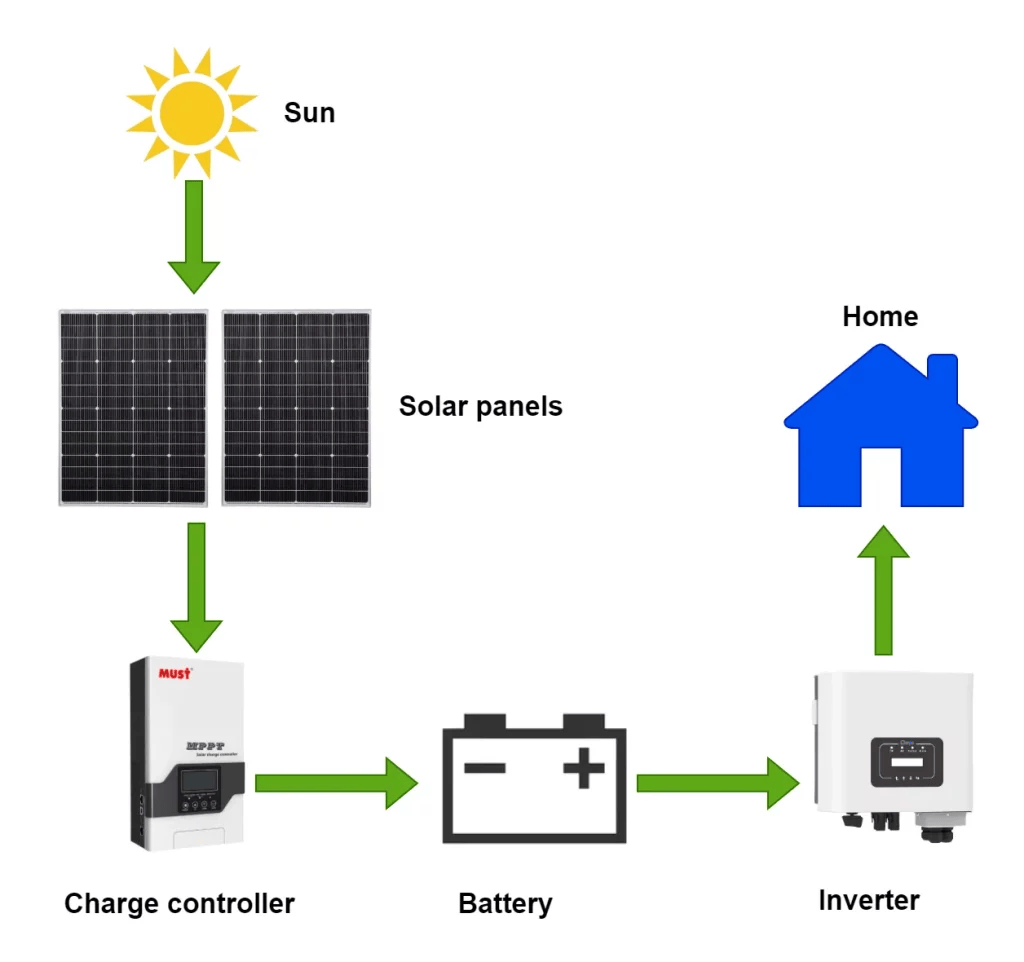
\includegraphics[width=0.4\textwidth]{figures/chap1/solar-system.png}
    \caption{Schematic of a Photovoltaic System}
    \label{fig:pv-system}
\end{figure}

\subsection{The Photovoltaic Effect}
\label{sec:pv-effect}

The photovoltaic effect, first observed by Edmond Becquerel in 1839, occurs when absorbed photons generate electron--hole pairs in a semiconductor p--n junction \citep{wurfel2016physics}. In silicon solar cells, this junction is formed by joining n-type and p-type regions, creating an internal electric field that separates photogenerated carriers and produces an external current under illumination \citep{marques2022photovoltaic}. Figure~\ref{fig:pv-effect} illustrates this principle \citep{energyeducation_pveffect}. The illuminated cell can be modeled by:
\begin{equation}
I = I_{\text{L}} - I_{0} \left[ \exp\left( \frac{q(V + I R_{\text{s}})}{n k_{\text{B}} T} \right) - 1 \right] - \frac{V + I R_{\text{s}}}{R_{\text{sh}}}
\label{eq:single-diode}
\end{equation}
where $I_{\text{L}}$ is the photocurrent, $I_{0}$ the dark saturation current, $n$ the ideality factor, $k_{\text{B}}$ the Boltzmann constant, $T$ the absolute temperature, $q$ the elementary charge, and $R_{\text{s}}$ and $R_{\text{sh}}$ the series and shunt resistances. This model is widely used in photovoltaic research because its five parameters ($I_{\text{L}}$, $I_{0}$, $n$, $R_{\text{s}}$, $R_{\text{sh}}$) can be extracted from measured I--V curves and serve as indicators of cell health and degradation \citep{alezz2022photovoltaic}.

\begin{figure}[H]
    \centering
    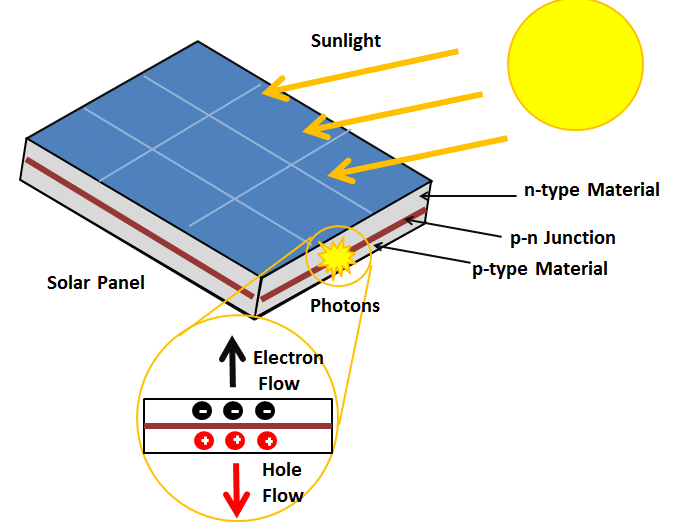
\includegraphics[width=0.4\textwidth]{figures/chap1/pv-effect.png}
    \caption{Photovoltaic Effect }
    \label{fig:pv-effect}
\end{figure}

\subsection{Components of a Photovoltaic System}
\label{sec:pv-components}

A photovoltaic system comprises several functional components designed to capture, regulate, convert, and distribute electrical energy safely \citep{franklinSolarPhotovoltaicPV}. The main components are detailed below.

\textbf{Solar Modules and Arrays:} The solar module is the foundational element that captures sunlight using multiple interconnected mono-crystalline or poly-crystalline silicon cells. To meet higher voltage and power requirements, several modules are wired together in series and parallel configurations to form a larger solar array.

\begin{figure}[H]
    \centering
    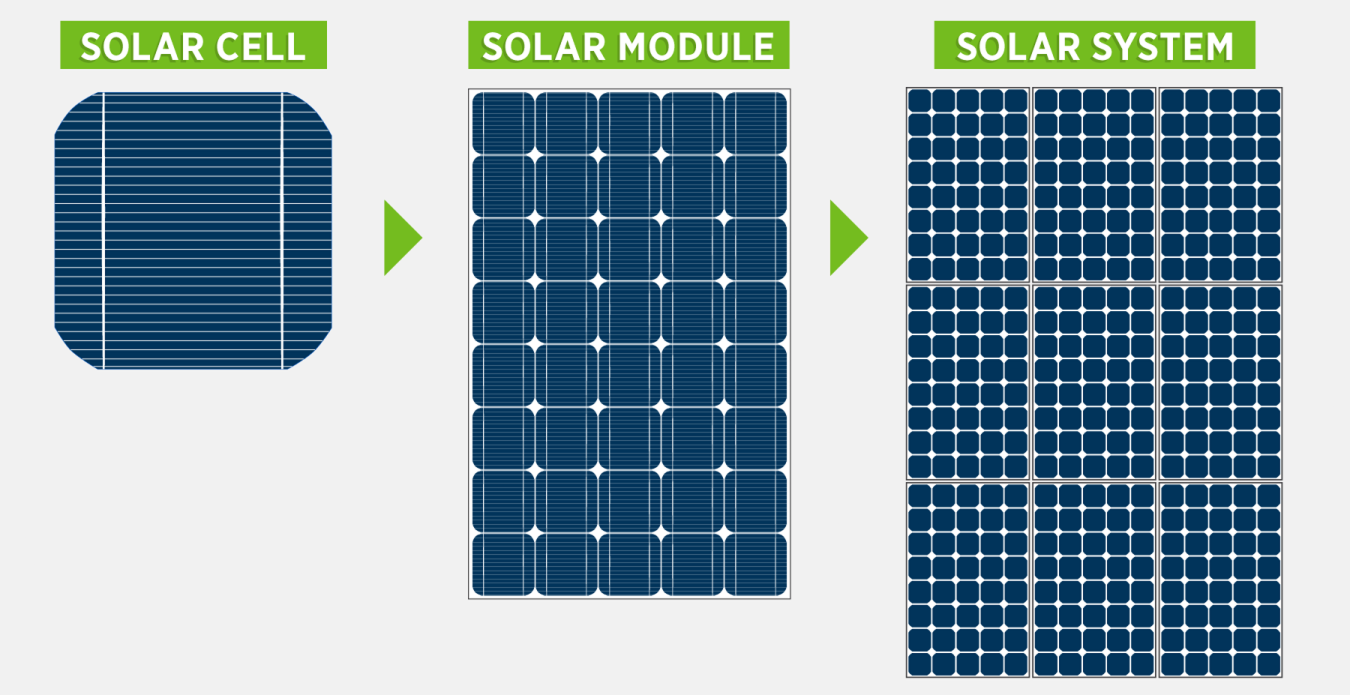
\includegraphics[width=0.4\textwidth]{figures/chap1/solar-module.png}
    \caption{The solar cell, module and array hierarchy \citep{doe2019pvcells101}}
    \label{fig:pv-components}
\end{figure}

\textbf{Combiner Box:} This electrical enclosure aggregates multiple series strings of solar modules into a single parallel output circuit. By consolidating these connections, the combiner box efficiently increases the total system current while maintaining the accumulated voltage of the strings.

\begin{figure}[H]
    \centering
    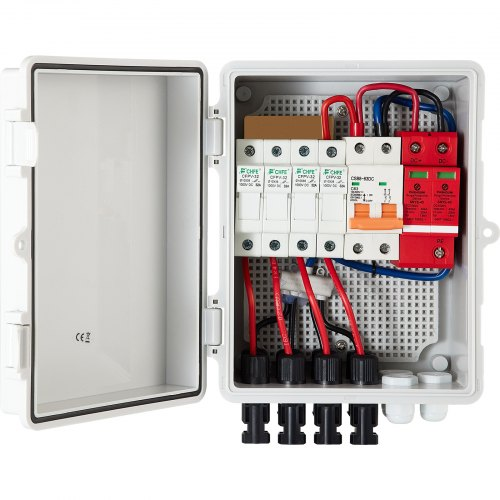
\includegraphics[width=0.3\textwidth]{figures/chap1/combiner-box.png}
    \caption{VEVOR PV Combiner Box for 4 Strings}
    \label{fig:combiner-box}
\end{figure}

\textbf{Charge Controller:} Positioned between the solar array and the battery bank, the charge controller regulates the incoming direct current. It plays a critical role in preventing battery overcharging and excessive discharging, thereby safely extending the operational lifespan of the storage system.
\begin{figure}[H]
    \centering
    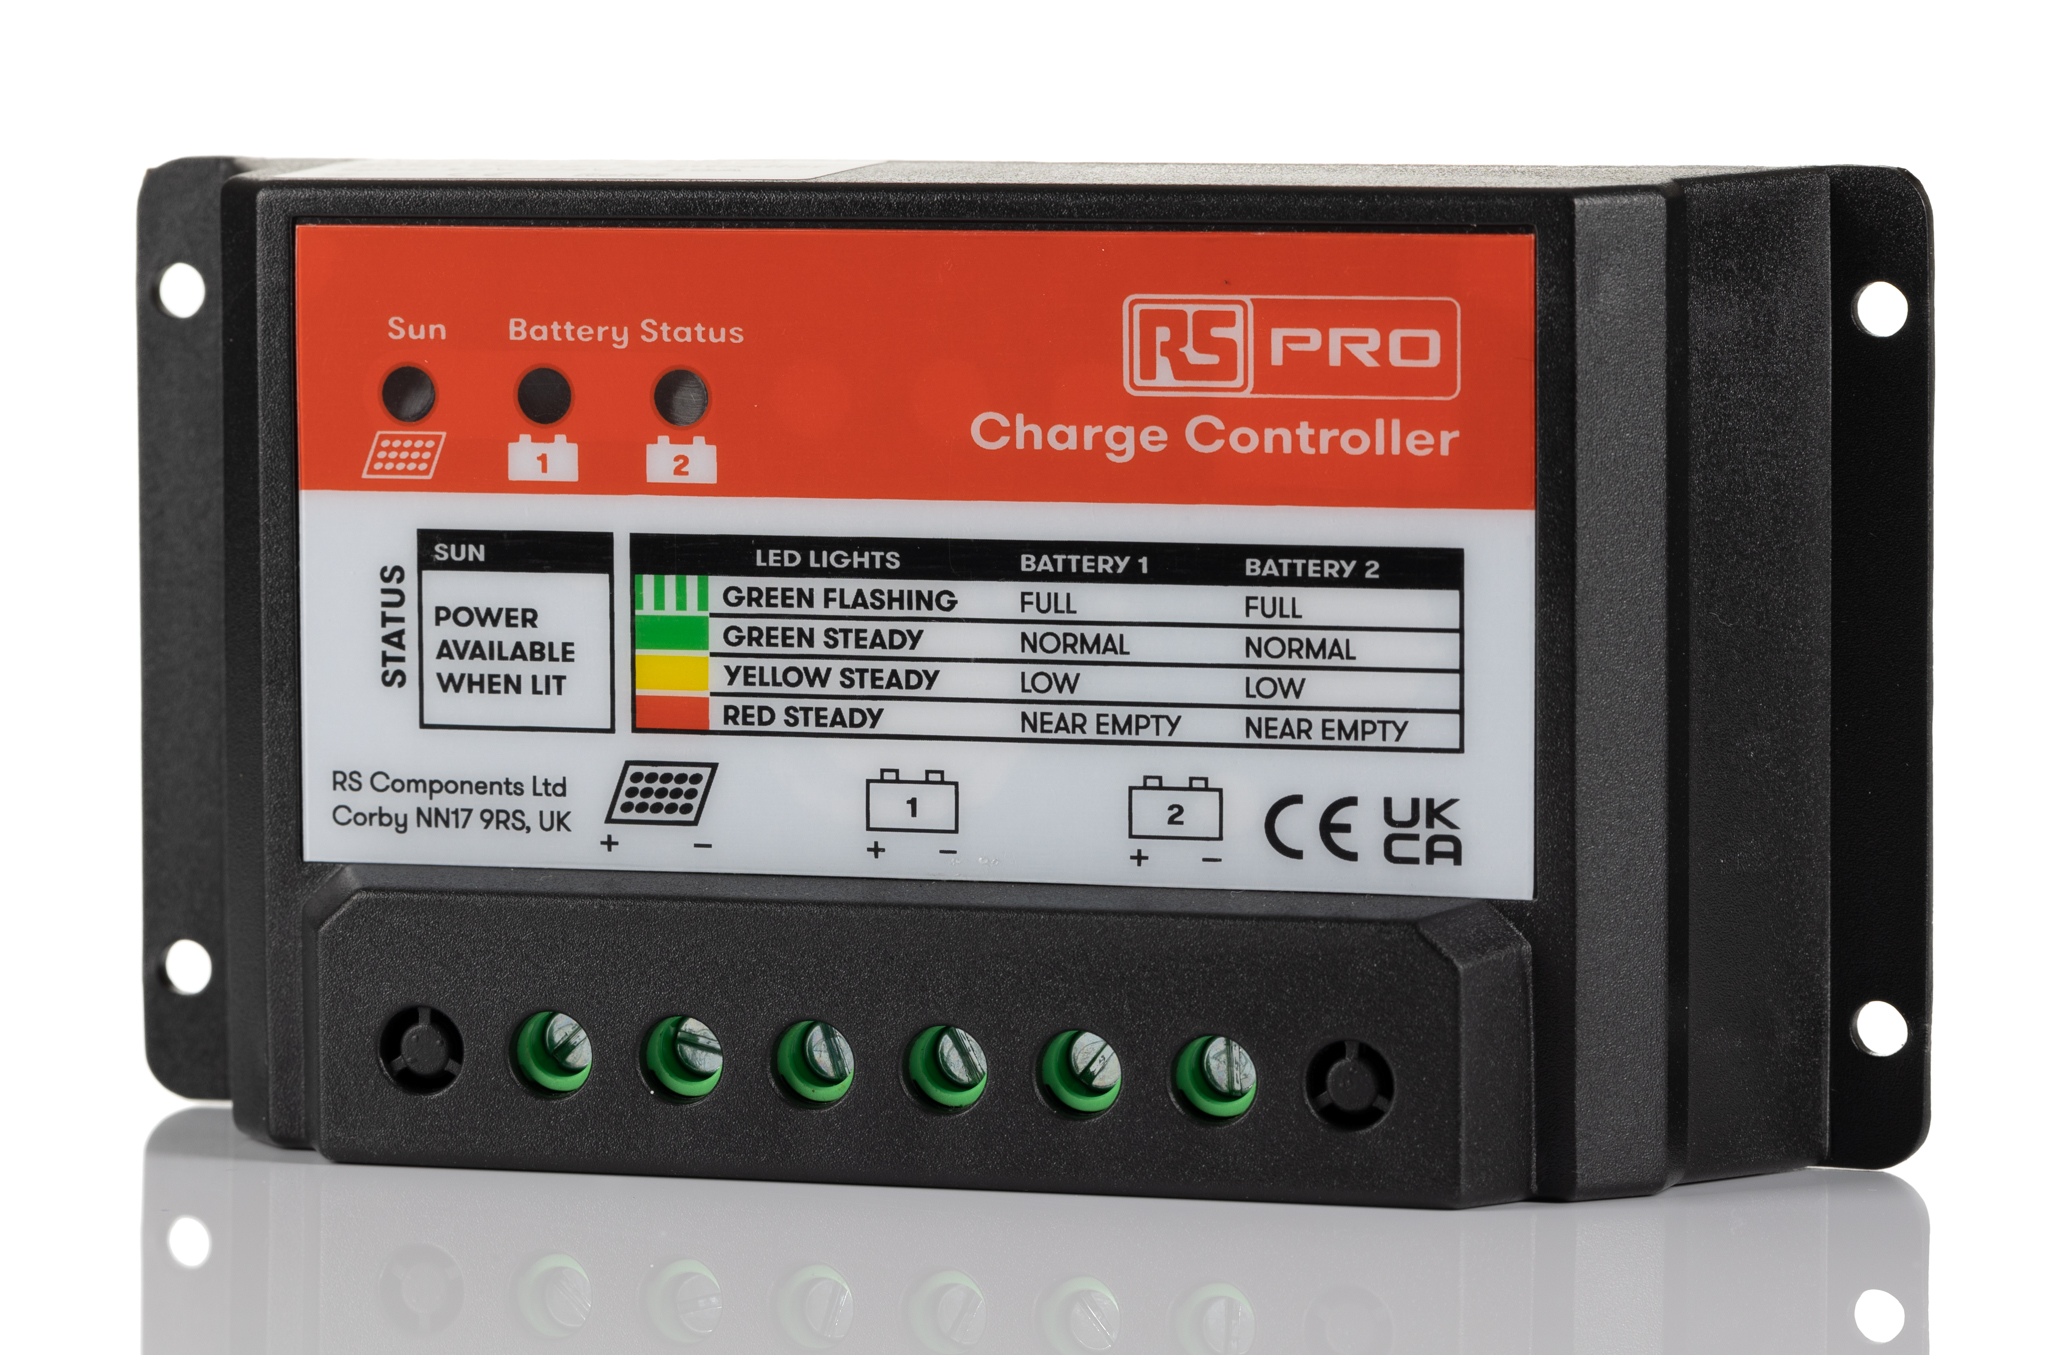
\includegraphics[width=0.3\textwidth]{figures/chap1/charge-controller.png}
    \caption{RS PRO Solar Charge Controller (24V/10A)}
    \label{fig:charge-controller}
\end{figure}
\textbf{Battery Bank:} In systems requiring energy storage, deep-cycle lead-acid batteries are utilized to store the electrical power produced during sunny periods. These batteries provide a reliable energy reserve to continuously power electrical loads during the night or periods of low solar irradiance.

\textbf{Inverter:} The inverter is a crucial power electronics device that converts the direct current generated by the array or stored in batteries into alternating current (AC). This conversion is essential because most residential and commercial electrical loads, as well as the external utility grid, operate exclusively on alternating current.
\begin{figure}[H]
    \centering
    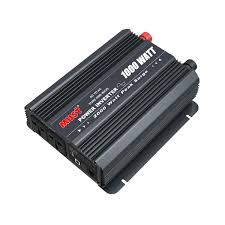
\includegraphics[width=0.3\textwidth]{figures/chap1/inverter.png}
    \caption{PI1500 Solar Power Inverter (120V 1000W)}
    \label{fig:inverter}
\end{figure}
\textbf{Disconnect Switches and Breakers:} Direct and alternating current disconnect switches are installed to safely isolate the power sources and the inverter during routine maintenance. These safety mechanisms ensure that the system can be completely de-energized, protecting the functional equipment and the maintenance personnel.

\subsection{Surveillance Systems}
\label{sec:pv-surveillance}
In the PV context, survillance systems refer to the integrated hardware and software tools used to collect and monitor system data, including electrical and meteorological parameters. These system are generally composed of sensors, plus a Supervisory Control and Data Acquisition (SCADA) system that collects, processes, and visualizes the data for performance monitoring and fault detection purposes \citep{taylorEffectivenessSCADASystem2020}.

A SCADA system typically includes Feild Devices (sensors and actuators), the main sensors in a PV system are a Pyranometer to measure solar irradiance, a Thermometer for ambient temperature and an Anemometer for wind speed measurement. Electrical parameters such as voltage, current, and power are measured directly from inverters. Remote Terminal Units are responsible for gathering data from sensors,
Master Terminal Units act as central nodes, collecting data from RTUs and providing interfaces for human operators. The collected data is also stored in a database for historical analysis \citep{yadavArchitectureSecuritySCADA2021}. An example of a SCADA system for PV monitoring can be seen in Figure~\ref{fig:scada-pv}.

\begin{figure}[H]
    \centering
    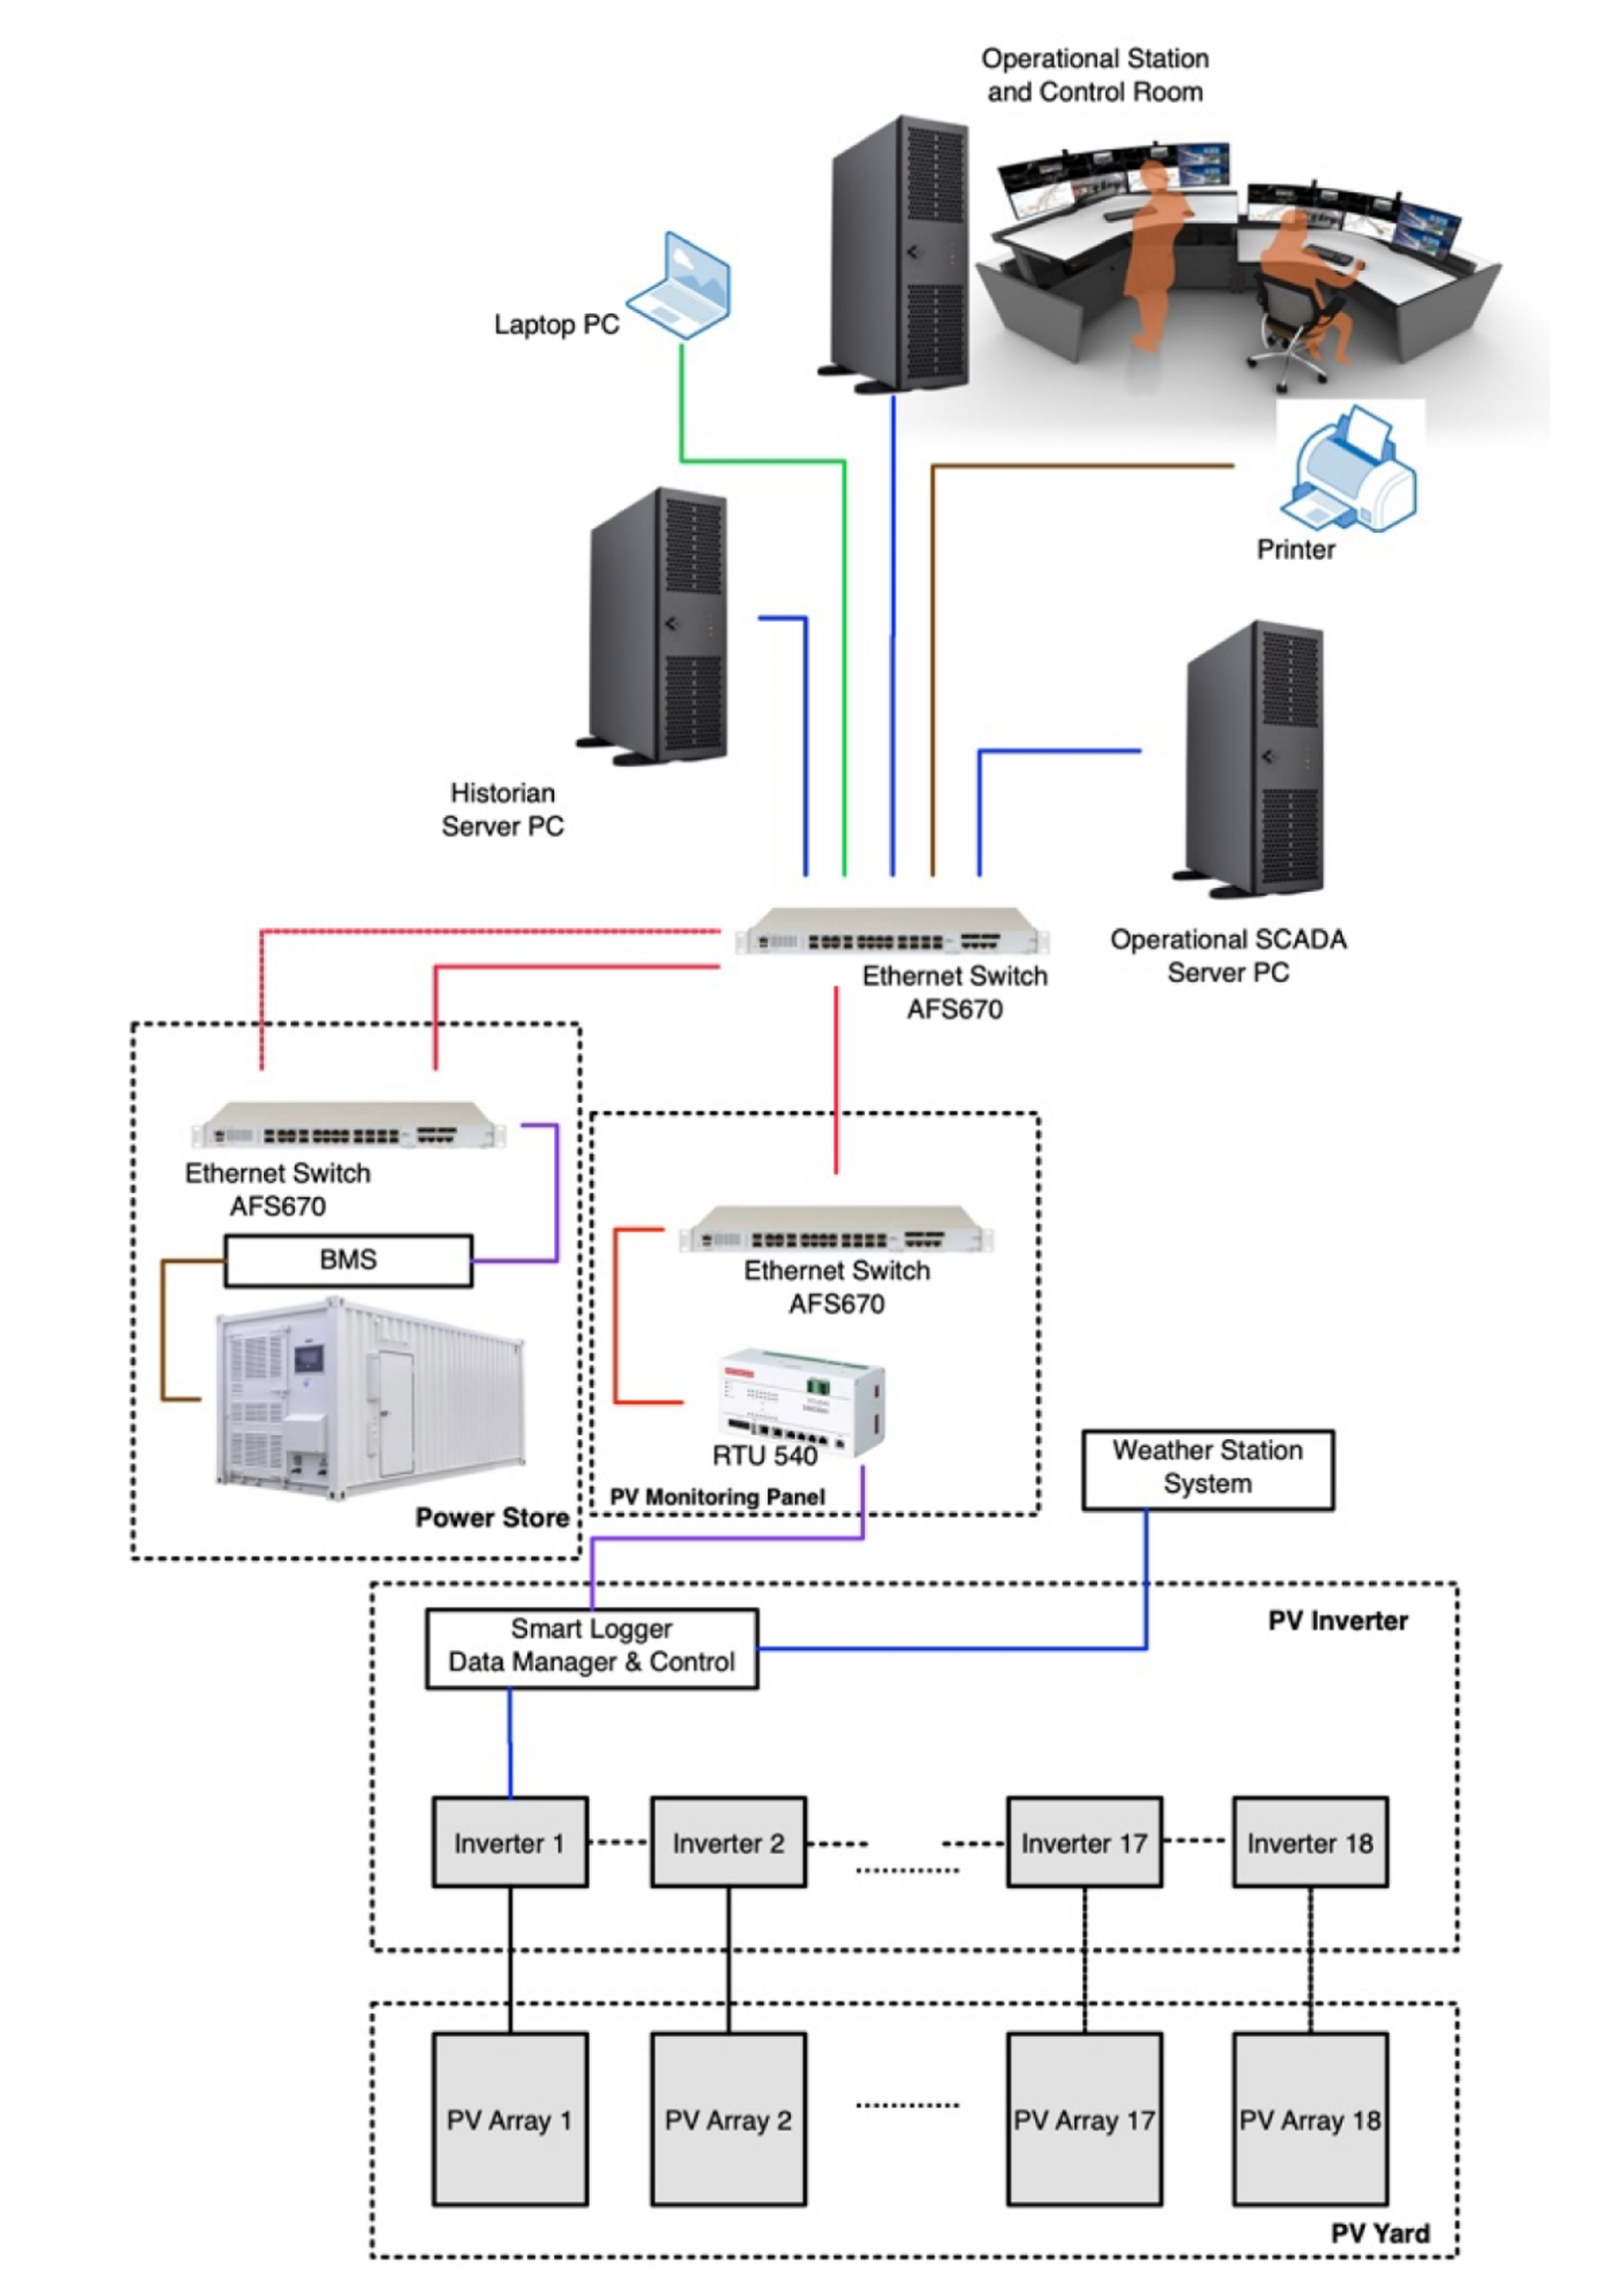
\includegraphics[width=0.7\textwidth]{figures/chap1/SCADAex.png}
    \caption{SCADA system for PV monitoring \citep{syamsuddinPredictiveMaintenanceBased2024}}
    \label{fig:scada-pv}
\end{figure}

\subsection{Global Operation of a Photovoltaic System}
\label{sec:pv-global-operation}

The operation of a photovoltaic system begins with the conversion of solar irradiance into 
direct current at the cell and module levels. Modules are interconnected into strings and 
arrays to achieve the required voltage and power levels. The generated DC power passes 
through protection and aggregation devices, and may be regulated by a charge controller 
when energy storage is used. An inverter then converts the DC power into alternating 
current for AC loads or grid injection. System operation is continuously monitored 
through sensors and SCADA platforms, which collect meteorological and electrical 
measurements for performance supervision and fault detection.


\section{Faults in PV Systems}
\label{sec:pv-faults}

Faults in a photovoltaic systems are any abnormal condition or physical damage causing operational parameters
to deviate from their normal range, leading to reduced performance, safety hazards, or system failure.
These anomalies can be grouped into different categories based on their different characteristics. \citep{elbanbyPhotovoltaicSystemFault2023} classified them into infant failures, mid-life 
failures and wear-out failures. While \citep{ArtificialIntelligenceInternet2021} categorized them into temporal and permanent faults. \citep{ComparativeAnalysisSolar2022} divided them into AC side 
faults and DC side faults. Down below are the most pertinent faults that can occur in a PV system:
\begin{itemize}
    \item \textbf{Open Circuit Fault:} Caused by a break in electrical continuity due to damaged cables, connectors, or fuses, leading to loss of power generation in the affected string.

    \item \textbf{Short Circuit Fault:} Occurs when unintended low-impedance paths form between conductors or to ground, producing abnormal current flow and safety risks.

    \item \textbf{Mismatch Fault:} Results from differences in module electrical characteristics caused by defects, degradation, or non-uniform operating conditions such as partial shading.

    \item \textbf{Hotspot Fault:} Appears when a cell operates in reverse bias and dissipates energy as heat, potentially causing permanent thermal damage.

    \item \textbf{Bypass Diode Fault:} Arises when a bypass diode fails, either reducing module output in short-circuit mode or increasing hotspot risk in open-circuit mode.

    \item \textbf{Shading Fault:} Produced by partial obstruction of sunlight, creating current imbalance between illuminated and shaded cells.

    \item \textbf{Soiling Fault:} Caused by dust or dirt accumulation on module surfaces, reducing irradiance absorption and power generation.

    \item \textbf{Thermal Stress Fault:} Results from prolonged high temperatures that accelerate aging and degradation of module materials and interconnections.

    \item \textbf{Inverter Fault:} Occurs when the power conversion stage malfunctions, affecting DC/AC conversion, cooling, or maximum power point tracking.
\end{itemize}

% Chapter 3: Related Work (USER)
% ============================================================
% Chapter 3: Related Work
% ============================================================
\chapter{Related Work}
\label{ch:related-work}

The field of fault detection and diagnosis in photovoltaic systems has attracted growing research interest over the past decade, driven by the rapid expansion of solar installations and the corresponding need for reliable automated monitoring solutions. This chapter reviews the existing literature with the objective of situating the contributions of this work within the current state of the art. The review is organized around three distinct families of diagnostic approaches, differentiated by the type of input data they exploit: thermographic imaging, current-voltage characteristic curve analysis, and operational electrical and meteorological measurements. Before examining these methodological families, it is necessary to characterize the datasets available in the field, as the nature of the training data fundamentally conditions the validity of performance claims and the generalizability of the proposed models. The chapter closes with a critical synthesis of the identified limitations and a statement of the research gaps that motivate the contributions of this thesis.

% ────────────────────────────────────────────────────────────
\section{Existing Datasets in Photovoltaic Fault Detection and Diagnosis}
\label{sec:datasets}
% ────────────────────────────────────────────────────────────

The availability of labeled, high-quality data is the foundational prerequisite for any supervised or semi-supervised learning approach to PV fault diagnosis. A comprehensive survey of open datasets for assessing PV system reliability highlights a striking asymmetry in the current data landscape: fault-labeled datasets are rare, and those that exist are predominantly generated under controlled laboratory conditions or through circuit simulation rather than collected from operational field installations \citep{chen2025datasets}. This section surveys the main publicly available datasets used in the literature reviewed in this chapter and identifies the principal limitations of the current data ecosystem.

Among the fault-labeled datasets based on real field measurements, two stand out for their quality and relevance to the operational scenario addressed in this thesis. The Costa dataset, introduced by \citet{costa2020sensors}, was collected from a 5~kW two-string grid-connected PV installation located in Brazil. Measurements were acquired at a sampling rate of 1~Hz over a 16-day campaign during which four distinct fault conditions were artificially induced in a controlled and reproducible manner: short-circuit faults, module degradation, open-circuit faults, and natural partial shading events. The resulting dataset contains approximately 516,000 labeled samples covering five operating states, with DC voltage, DC current, solar irradiance, and module temperature as the primary measurement channels. Because faults were induced by physically modifying the installation rather than simulated numerically, the dataset captures genuine electrical transients and retains the measurement noise and environmental variability inherent to outdoor operation. This combination of labeling rigor and real-world grounding makes the Costa dataset a valuable reference benchmark for data-driven FDD research.

The La Réunion dataset, collected from a grid-connected PV installation on the French island of La Réunion, represents a complementary real-world resource. Unlike the Costa dataset, whose faults were deliberately induced by the experimenter, the La Réunion dataset contains faults that occurred naturally during prolonged field operation, resulting in a fault rate of approximately 3\% of total observations and a strong dominance of shading-related fault classes. The dataset comprises approximately three million timestamped records sampled at an interval of roughly seven seconds, and the available fault labels are organized into a hierarchical taxonomy covering several variants of partial shading effects. The high class imbalance and the restriction to a single fault family make this dataset substantially more challenging than Costa for classification purposes and more representative of the conditions encountered in actual PV plant monitoring.

In the simulated domain, the GPVS-Faults dataset \citep{bakdi2021gpvs}, available through the Mendeley data repository, provides labeled measurements generated from a grid-connected PV system emulated in a laboratory environment at a sampling rate of 100~kHz. The dataset encompasses eight fault scenarios spanning both array-level and inverter-level faults, organized across sixteen experimental files corresponding to two operating modes: maximum power point tracking (MPPT) and imposed power point tracking (IPPT). The high sampling rate and diversity of fault types make this dataset useful for evaluating signal processing approaches, particularly those based on spectral decomposition. However, the absence of meteorological channels and the controlled laboratory conditions mean that the dataset does not capture the environmental variability that characterizes real PV operation.

Beyond these three primary datasets, the broader PV monitoring community has produced a number of performance datasets that, while lacking fault labels, represent valuable resources for representation learning and transfer learning purposes. The PVDAQ database, maintained by the National Renewable Energy Laboratory, aggregates operational measurements from 158 PV installations across the United States spanning periods of one to twenty-nine years at resolutions of fifteen minutes or finer \citep{pvdaq2023}. The SKIPP'D dataset provides one-minute power generation records from a 30~kW rooftop installation alongside sky camera images, enabling research at the intersection of visual and electrical monitoring \citep{skipd2023}. The scientific community has also proposed fully simulated datasets with finer fault taxonomies; the dataset introduced by \citet{srisiri_artificial_2025} covers 17 fault classes across more than 12,000 simulated samples, offering greater class diversity at the cost of physical realism. Table~\ref{tab:datasets} summarizes the main characteristics of the datasets discussed in this section.

\begin{table}[htbp]
\centering
\caption{Summary of publicly available datasets for PV fault detection and diagnosis. SC: short-circuit; OC: open-circuit; Deg: degradation; Shad: partial shading.}
\label{tab:datasets}
\begin{tabular}{lllllr}
\toprule
\textbf{Dataset} & \textbf{Type} & \textbf{Rate} & \textbf{Fault Labels} & \textbf{Fault Classes} & \textbf{Size} \\
\midrule
Costa (2020)            & Real, field    & 1 Hz       & Yes & SC, OC, Deg, Shad (4)    & 516k rows  \\
La Réunion              & Real, field    & 0.14 Hz    & Yes & Shading variants (7)      & 3M rows    \\
GPVS-Faults (Mendeley)  & Lab simulated  & 100 kHz    & Yes & Array + inverter (8)      & 16 files   \\
Srisiri et al. (2025)   & Simulated      & ---        & Yes & Multi-type (17)           & 12,835     \\
PVDAQ (NREL)            & Real, field    & 15 min     & No  & ---                       & 158 sites  \\
SKIPP'D                 & Real, rooftop  & 1 min      & No  & ---                       & 3 years    \\
\bottomrule
\end{tabular}
\end{table}

The picture that emerges from this survey is one of significant data scarcity. The number of publicly available, fault-labeled datasets based on genuine field measurements remains extremely limited, and those that exist cover a narrow range of climatic conditions, PV technologies, and fault types. This scarcity has pushed a substantial fraction of the research community toward simulated data, which introduces a fundamental validity concern: models that achieve high diagnostic accuracy on numerically generated data may fail to generalize when confronted with the sensor imperfections, environmental variability, and installation-specific behavior of real PV systems. This tension between data accessibility and generalization validity constitutes one of the central challenges that this thesis addresses.

% ────────────────────────────────────────────────────────────
\section{Thermal Image-Based Fault Detection}
\label{sec:thermal}
% ────────────────────────────────────────────────────────────

Infrared thermography has been widely adopted as a diagnostic modality in PV fault detection research, primarily for its ability to reveal hotspot anomalies that are invisible to conventional optical inspection. In a healthy PV module, the temperature distribution across the cell surface is approximately uniform under steady irradiance conditions. Faults such as shading, cell cracking, bypass diode failures, and soiling create localized thermal dissipation patterns that manifest as temperature differentials detectable by infrared cameras. The diagnostic pipeline for thermographic approaches typically involves acquiring aerial images of PV arrays using unmanned aerial vehicles (UAVs) equipped with thermal sensors, applying image preprocessing to normalize illumination and correct geometric distortions, and then feeding the processed images into a classification model.

Convolutional neural networks (CNNs) have become the dominant model family for thermographic fault diagnosis, owing to their proven ability to extract spatially local features from image data. \citet{manno2021thermal} proposed a deep learning framework that leverages convolutional feature extraction applied directly to thermographic images of PV modules, achieving classification accuracies exceeding 95\% across several fault categories including hotspots, cell cracks, and diode failures on images collected from a real installation. \citet{gong2024deep} developed a method based on adaptive deep multiscale feature enhancement to handle significant variation in hotspot sizes and thermal contrast levels across different imaging conditions, reporting fast detection times suitable for online monitoring scenarios. More recently, hybrid approaches have combined thermal imaging with other modalities; \citet{ettaleby2022fault} integrated K-means clustering on thermal images with coded wireless OFDM signal processing to improve fault localization precision beyond what pure image analysis can achieve.

Despite these results, thermographic approaches carry two fundamental limitations that restrict their applicability in large-scale operational deployment. The first is the cost and logistics of the acquisition infrastructure. Generating thermographic images at the resolution required for reliable hotspot detection requires calibrated infrared cameras, which are substantially more expensive than standard silicon-based sensors. When combined with UAVs capable of carrying such payloads and the flight operations required to systematically survey a utility-scale installation, the per-inspection cost becomes prohibitive for routine continuous monitoring. The second limitation is the temporal resolution of the diagnostic process. Thermographic surveys are inherently event-driven and infrequent: a fault that develops between inspection campaigns may propagate for weeks or months before detection. These two constraints together mean that thermographic methods, despite their effectiveness within their domain of applicability, are not suitable as the primary monitoring modality for installations requiring near real-time fault awareness at low operational cost.

% ────────────────────────────────────────────────────────────
\section{Current-Voltage Curve-Based Fault Detection}
\label{sec:ivcurve}
% ────────────────────────────────────────────────────────────

The current-voltage (I-V) characteristic curve of a PV module encodes its complete electrical behavior at a given irradiance and temperature. Under healthy operating conditions, this curve follows a well-defined shape governed by the single-diode model: a plateau of quasi-constant current at low voltages, a knee region near the maximum power point, and a steep decline to zero at the open-circuit voltage. Different fault types produce characteristic distortions of this shape that serve as discriminative signatures. Partial shading introduces step-like discontinuities in the curve as successive bypass diodes activate. Increased series resistance tilts the slope of the knee region and reduces the fill factor. Decreased shunt resistance raises the slope of the plateau region near the short-circuit current. These predictable deformations have motivated a family of diagnostic approaches based on I-V curve measurement and analysis.

Machine learning methods applied to extracted I-V features have demonstrated consistently high performance in controlled settings. \citet{chen2017} proposed a kernel extreme learning machine trained on a set of features derived from the I-V curve, including the short-circuit current, the open-circuit voltage, the maximum power point coordinates, and the fill factor, reporting fault diagnosis accuracies above 93\% across multiple fault types on a simulated dataset. \citet{eskandari2020} applied an ensemble learning approach to line-to-line fault detection, using I-V and P-V curve features to distinguish between healthy operation and various fault configurations and achieving classification accuracy exceeding 95\%. Deep learning approaches have extended this paradigm by bypassing manual feature extraction. \citet{liu2021sae} used a stacked autoencoder to learn a latent representation of the I-V curve directly and then applied clustering to group measurements into fault categories without requiring labeled training data. \citet{qu2024dust} proposed transforming I-V curves into graphical image representations and applying CNNs augmented with convolutional block attention modules (CBAM) to perform fault classification under varying soiling and dust conditions, achieving results above 99\% on both simulated and experimental data.

The central limitation of I-V curve-based approaches lies in the measurement procedure itself. Acquiring a full I-V sweep requires varying the load applied to the PV module or string across its full operating range, temporarily interrupting normal power generation. In large-scale installations comprising thousands of modules organized into multiple strings, performing systematic I-V measurements on each module at regular intervals is logistically complex, time-consuming, and operationally intrusive. Furthermore, the measurement accuracy of I-V sweeps is sensitive to rapid changes in irradiance and temperature during the sweep duration, introducing uncertainty that can mask subtle fault signatures. These constraints make I-V curve analysis more suitable as a periodic diagnostic complement than as a primary real-time detection modality.

% ────────────────────────────────────────────────────────────
\section{Electrical and Meteorological Data-Based Methods}
\label{sec:elec-meteo}
% ────────────────────────────────────────────────────────────

The third and most practically relevant family of data-driven PV fault detection methods operates on the operational electrical and meteorological measurements that modern PV installations continuously generate as part of their standard monitoring infrastructure. These measurements, including DC voltage and current at the string level, AC power at the inverter output, solar irradiance, and module and ambient temperatures, are already collected by dataloggers and SCADA systems in most grid-connected PV plants without any additional sensing hardware. This key advantage makes electrical and meteorological data-based approaches the most scalable option for continuous, near real-time fault monitoring.

\subsection{Machine Learning Approaches}

Classical machine learning methods were among the first to be applied to PV fault detection using operational electrical data, and they remain competitive with more recent deep learning approaches on tabular, low-frequency measurement data. \citet{garoudja2017ml} demonstrated that combining statistical process control techniques with supervised classifiers applied to real electrical measurements suffices to distinguish between the most common fault conditions in a grid-connected installation. Support vector machines have been extensively studied for this task; \citet{suliman2024ml} evaluated multiple SVM kernel configurations on electrical fault data and demonstrated that properly tuned SVMs achieve classification accuracies above 95\% on binary and multi-class fault problems. Random forests have also shown strong performance: \citet{amiri2024rf} trained a random forest classifier on features extracted from the DC measurements of a real PV system, reporting diagnostic accuracy exceeding 98\% on a balanced evaluation set and demonstrating the robustness of ensemble methods to field measurement noise.

Gradient boosting algorithms have demonstrated remarkable effectiveness on tabular PV fault data. \citet{noura_explainable_2025} proposed a two-phase fault detection and diagnosis framework based on Extra Trees, achieving detection accuracy of 99.5\% and diagnosis accuracy of 98.7\% while integrating explainability through SHAP and LIME analyzers. \citet{kull_adaptive_2025} combined a Deep Belief Network for feature extraction with LightGBM for classification on a real-world SCADA dataset from a 100~MW solar facility, achieving 98.21\% accuracy on a seven-class problem. The study by \citet{zwirtes_fault_2025} is particularly relevant for generalization: the authors trained multiple ML classifiers on two real PV installations with different module characteristics and found that models trained on one system face significant performance degradation when applied to the other, underscoring the installation-specific nature of fault signatures. Unsupervised and semi-supervised approaches address the label scarcity problem that limits fully supervised methods; \citet{kabir_isolation_2023} applied Isolation Forest to PV operational data and demonstrated its effectiveness for detecting anomalous patterns without requiring labeled fault examples, while \citet{qu2022unsupervised} combined unsupervised weather pattern recognition with blending fitting models to enable label-free fault detection.

\subsection{Deep Learning Approaches}

Deep learning methods enable the automatic extraction of temporal and structural features from raw time-series measurements, reducing dependence on manual feature engineering. \citet{amiri2024dl} proposed a hybrid architecture combining one-dimensional convolutional feature extraction with a bidirectional GRU for fault detection and diagnosis in a real PV system, demonstrating that the combination of spatial and temporal feature extraction outperforms either component alone with near-perfect accuracy on their evaluation dataset. Autoencoder-based architectures have attracted particular interest for the anomaly detection task, where the goal is to learn a compact representation of normal operating behavior and flag deviations as fault events. \citet{seghiour2023autoencoder} trained a deep autoencoder exclusively on normal operation data and demonstrated that reconstruction error is a reliable anomaly score for identifying fault conditions even without labeled fault examples. \citet{titouni_hybrid_2025} extended this principle with a hybrid CNN-Autoencoder architecture evaluated on the GPVS-Faults dataset, achieving 98.84\% test accuracy and outperforming several benchmark architectures. The Adaptive PolyKAN Autoencoder of \citet{attouri_adaptive_2026} combined polynomial kernel networks with an autoencoder for dimensionality reduction, reducing computational overhead by over 88\% while preserving diagnostic accuracy above 96\%.

Attention mechanisms and Transformer architectures have begun to penetrate this domain. \citet{khalil2024transformer} applied a Transformer model to fault classification in PV systems, leveraging multi-head self-attention to capture long-range dependencies in electrical time-series and achieving 95.8\% accuracy across multiple fault types. Graph-based methods represent a newer direction: \citet{yan_som-dbtgnet_2025} introduced SOM-DBTGNet, combining self-organizing maps for anomaly score generation with a dual-branch temporal graph convolution network that explicitly models topological relationships between measurement channels, achieving 90.7\% accuracy across six fault categories. Signal processing hybrid approaches further enrich the electrical modality: \citet{cai2022arc} used variational mode decomposition to decompose string current signals into intrinsic mode functions before applying a PSO-tuned SVM, enabling reliable detection of arc fault signatures invisible in raw time-domain measurements; wavelet transforms have similarly been applied as preprocessing for SCADA-based fault detection, particularly for faults with fast transient dynamics \citep{saiprakash_improved_2024}.

% ────────────────────────────────────────────────────────────
\section{Synthesis and Comparative Analysis}
\label{sec:synthesis}
% ────────────────────────────────────────────────────────────

The preceding review reveals a landscape of considerable methodological diversity, where each input modality and model family presents distinct strengths and limitations. Table~\ref{tab:synthesis} consolidates a representative selection of reviewed works along the dimensions most relevant to practical deployment assessment.

\begin{table}[htbp]
\centering
\caption{Representative methods for PV fault detection and diagnosis reviewed in this chapter. R: real data; S: simulated data; N/S: not specified.}
\label{tab:synthesis}
\small
\begin{tabular}{llllcl}
\toprule
\textbf{Author(s)} & \textbf{Year} & \textbf{Modality} & \textbf{Method} & \textbf{Data} & \textbf{Edge} \\
\midrule
Manno et al.       & 2021 & Thermal     & CNN                  & R    & No \\
Gong et al.        & 2024 & Thermal     & Multiscale CNN       & R    & No \\
Chen et al.        & 2017 & I-V curve   & Kernel ELM           & S    & No \\
Eskandari et al.   & 2020 & I-V curve   & Ensemble learning    & S    & No \\
Qu et al.          & 2024 & I-V curve   & CNN-CBAM             & R+S  & No \\
Garoudja et al.    & 2017 & Electrical  & SVM + SPC            & R    & No \\
Amiri et al.       & 2024 & Electrical  & Random Forest        & R    & No \\
Noura et al.       & 2025 & Electrical  & Extra Trees + XAI    & S    & No \\
Kull et al.        & 2025 & Electrical  & DBN + LightGBM       & R    & No \\
Seghiour et al.    & 2023 & Electrical  & Autoencoder          & S    & No \\
Amiri et al.       & 2024 & Electrical  & CNN + Bi-GRU         & R    & No \\
Khalil et al.      & 2024 & Electrical  & Transformer          & S    & No \\
\bottomrule
\end{tabular}
\end{table}

Several patterns emerge from this synthesis. First, reported accuracies are consistently high across all modalities and method families, frequently exceeding 95\% and often approaching 100\%. While these figures reflect genuine technical progress, they must be interpreted with caution given that many studies rely on simulated data, use small or class-balanced evaluation sets, or apply validation protocols that do not adequately guard against temporal data leakage. Second, the electrical and meteorological modality is the most extensively represented in the literature, consistent with the observation that operational electrical measurements are the most readily available data type in real PV installations. Third, and most strikingly, not a single reviewed work incorporates an edge deployment constraint or reports inference performance on embedded hardware. The entire reviewed literature assumes unlimited computational budget and centralized processing infrastructure, an assumption increasingly at odds with the operational requirements of distributed PV monitoring systems.

% ────────────────────────────────────────────────────────────
\section{Research Gap and Motivation}
\label{sec:gap}
% ────────────────────────────────────────────────────────────

The preceding review, combined with the dataset landscape analyzed in Section~\ref{sec:datasets}, identifies five interconnected limitations in the existing literature that motivate the specific contributions of this thesis.

\textbf{The impracticality of specialized sensing modalities.} Thermographic approaches require infrared cameras and UAV logistics that are too costly and operationally disruptive for continuous real-time monitoring at scale. I-V curve methods require interrupting power generation and physically isolating modules, which is unfeasible for routine online monitoring of large arrays. These constraints restrict two of the three main diagnostic modalities to periodic, campaign-based inspections rather than continuous monitoring. The operational constraints of real PV plant management motivate an approach that relies exclusively on the electrical and meteorological measurements already produced by standard inverter and sensor infrastructure, enabling continuous monitoring at no additional hardware cost.

\textbf{The dominance of synthetic training data.} As evidenced by Table~\ref{tab:synthesis} and the dataset survey in Section~\ref{sec:datasets}, a significant fraction of the literature trains and evaluates models on data generated through circuit simulation or laboratory emulation. These settings do not capture the sensor noise, missing values, weather-driven nonlinearities, and installation-specific variability that characterize real field operation. As \citet{zwirtes_fault_2025} demonstrated, models trained on one real system can fail substantially when applied to another installation with different hardware characteristics. The high accuracy figures reported on clean simulated datasets are therefore not representative of real-world performance, and this gap motivates working with genuine field measurements from real PV installations.

\textbf{Limited fault diversity and the challenge of subtle faults.} Most reviewed studies address one to three fault types, and many restrict evaluation to faults with clearly discriminative electrical signatures such as short-circuit or open-circuit conditions. The degradation fault is notably underrepresented despite its practical importance: it manifests as a subtle, progressive reduction in module current that is difficult to distinguish from natural performance variability caused by environmental fluctuations. Reconstruction-based anomaly detection models are particularly prone to misclassifying mild degradation as normal operation because they learn to reconstruct the normal manifold and tend to reconstruct subtle deviations well. This limitation motivates an approach that explicitly handles a diverse set of four fault types, including the challenging degradation class, and evaluates diagnostic performance on a per-class basis rather than through aggregate accuracy metrics that can mask poor performance on specific fault categories.

\textbf{The absence of edge deployment constraints.} As shown in Table~\ref{tab:synthesis}, no reviewed work reports the deployment of a diagnostic model on embedded hardware or quantifies inference latency and memory footprint under realistic computational constraints. This represents a significant disconnect between research and practice: PV monitoring systems are increasingly expected to operate at the edge of the network, close to the data source, to minimize communication bandwidth requirements and enable local decision-making. Designing models with edge deployment constraints in mind from the outset, and validating them on resource-constrained hardware, constitutes a contribution that the existing literature has not addressed.

\textbf{The absence of lifecycle management and data drift handling.} PV system characteristics evolve over time as modules age, soiling patterns change seasonally, and environmental conditions shift. Static models trained once and deployed without updating mechanisms are inherently unable to adapt to this distribution shift, leading to gradual performance degradation that is difficult to detect without dedicated monitoring. The existing literature makes no provision for online adaptation, drift detection, or model retraining under operational conditions. An end-to-end pipeline incorporating drift detection mechanisms alongside the diagnostic model represents a practical contribution toward operationally robust PV fault monitoring.

% ────────────────────────────────────────────────────────────
\section*{Chapter Conclusion}
% ────────────────────────────────────────────────────────────

This chapter has reviewed the principal data-driven approaches to PV fault detection and diagnosis across three input modalities, characterized the available public datasets, and identified five research gaps in the existing literature. The review established that electrical and meteorological operational measurements represent the most practical and scalable diagnostic modality, that the scarcity of real-world labeled data constitutes a fundamental challenge for the field, and that the absence of edge deployment considerations in the existing literature creates a gap between reported research performance and practical operational requirements. Part~II of this document presents the contributions of this thesis, which directly address each of the identified limitations through a rigorous, reproducible pipeline applied to real PV field data and validated through deployment on an embedded Jetson Nano platform.


% ── Part II: Contributions ───────────────────────────────────
\part{Contributions}
% ============================================================
% Part II — Preface
% ============================================================

\newpage
\thispagestyle{plain}
\vspace*{2cm}

{\noindent\large\bfseries Part II — Contributions}

\vspace{1.2cm}

\noindent Part~I established the theoretical foundations of this work: the physics of photovoltaic systems and their failure modes, the machine learning and deep learning methods relevant to fault detection and diagnosis, and the state of the art that defines the open problems this work addresses. Part~II presents the original contributions.

\vspace{0.6cm}

\noindent Three contributions structure this part. First, a reproducible, leakage-controlled data pipeline is constructed and validated on two independent real-world field datasets, demonstrating architectural portability across distinct field sites. Second, both diagnostic tasks are evaluated at the per-class level, providing a fine-grained characterization of each method's diagnostic capability under real field conditions, beyond what aggregate metrics alone can reveal. Third, the complete system is deployed on a Jetson Nano edge platform with drift detection and on-device retraining, closing the loop between offline training and operational use.

\vspace{0.6cm}

\noindent \textbf{Chapter~\ref{ch:design}} defines the shared experimental infrastructure common to both tasks: the formal system model, the data pipeline, the splitting and preprocessing protocols, the feature engineering profiles, and the evaluation methodology.

\noindent \textbf{Chapter~\ref{ch:detection}} presents the anomaly detection task (Task~A): a semi-supervised formulation and a comparative evaluation across classical and deep learning methods.

\noindent \textbf{Chapter~\ref{ch:classification}} presents the fault classification task (Task~B): a multi-class tournament on real fault data, with a dedicated leakage validation of the headline result.

\noindent \textbf{Chapter~\ref{ch:deployment}} presents the edge deployment: ONNX model export, Jetson Nano benchmarks, the monitoring graphical interface, and the operational drift detection and on-device retraining loop.

\clearpage


\chapter{Design of a Fault Detection and Diagnosis System for Photovoltaic Systems}
\label{ch:conception}

\section{Introduction}

The process of designing a FDD system for photovoltaic systems involves several parts, including system architecture, dataset selection, data preprocessing, feature engineering, model selection and evaluation.
Each of these steps is cruicial to build a robust and effective FDD solution. The following sections will detail the design choices made for each step.

\section{System Architecture}
The overall architecture includes 4 main components, as illustrated in figure \ref{fig:system_architecture}:
\par\noindent\textbf{Data collection and transformation:} Collects raw data from sensors such as irradianceand ambient temperature, and electrical signals and applies the necessary preprocessing and transformations
to make it suitable for input to the next stage of the system.
\par\noindent\textbf{Anomaly Detection:} Upon receiving the preprocessed data, this component detects persistent deviations from expected values under observed meteorological conditions. Such deviations may indicate an anomaly in the system.
\par\noindent\textbf{Fault Diagnosis:} If an anomalt is detected, this component's responsability is to determine the type of fault that has occured from a pre-determined set of faults.
\par\noindent\textbf{Monitoring Interface:} Displays the system's real-time status, including detected anomalies, diagnosed faults along with their confidance scores, incoming data visualizations and performance rapports. 


\begin{figure}[H]
    \centering
    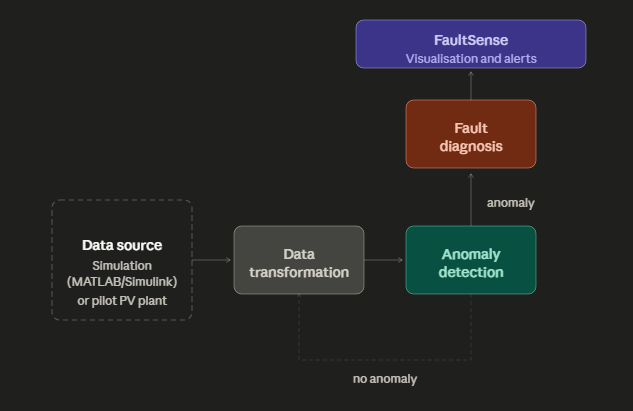
\includegraphics[width=0.8\textwidth]{figures/chap3/fdd-arch.png}
    \caption{FDD System Architecture.}
    \label{fig:system_architecture}
\end{figure}

\section{Dataset Selection}
Based on the previous dataset survey in\ref{sec:data-survey}, the Costa and La Réunion datasets were selected for the development and evaluation of our FDD system.
\textbf{Costa} is the primary experimental dataset, collected from a grid-connected pilot PV plant located in City of Curitiba-State of Paraná, Brazil. It contains 16 Canadian 330W Poly-crystalline Modules (CS6U-330P) divided into 2 strings of 8 modules each
running the Maximum Power Poin Tracking (MPPT) algorithm. The system may yeild 5kW peak installed capacity \citep{MonitoringSystemOnline2020}. The figure \ref{fig:costa_circuit} illustrates in detail the electrical configuration.
\begin{figure}[H]
    \centering
    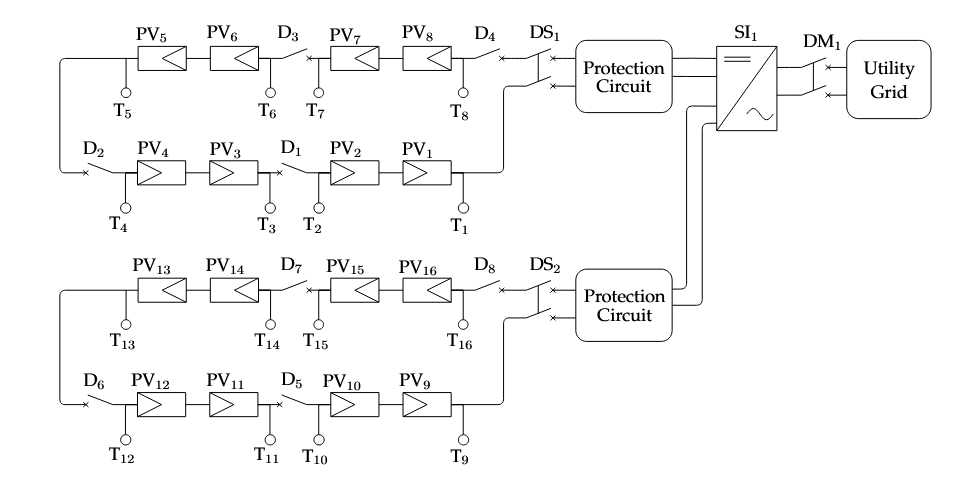
\includegraphics[width=0.8\textwidth]{figures/chap3/costa-shema.png}
    \caption{Costa Photovoltaic Plant Electrical Diagram \citep{MonitoringSystemOnline2020}.}
    \label{fig:costa_circuit}
\end{figure}

This dataset contains 4 fault types: \textbf{Shadowing}, \textbf{Degradation}, \textbf{Open-Circuit} and \textbf{Short-Circuit}. The full detail is illustrated in Table~\ref{tab:costa_label_counts}.

\begin{table}[H]
    \centering
    \caption{Number of data points in the Costa dataset.}
    \label{tab:costa_label_counts}
    \begin{tabular}{l r}
        \toprule
        Label & Number of data points \\
        \midrule
        Degradation & 10,371 \\
        Short-circuit & 5,999 \\
        Open-circuit & 6,024 \\
        Partial shadowing & 184,311 \\
        No fault introduced & 309,253 \\
        \midrule
        Total & 515,958 \\
        \bottomrule
    \end{tabular}
\end{table}

This dataset was chosen for its real-world nature which captures the noise and imperfections of actual PV system measurements, as well as its diverse fault types
and the presence of a large number of data points which allows for robust model training and evaluation. Additionally, the dataset includes both electrical and meteorological measurements. A full list of available features is provided in Table~\ref{tab:costa_features}.

\begin{table}[H]
    \centering
    \caption{Costa dataset features and descriptions.}
    \label{tab:costa_features}
    \begin{tabularx}{\textwidth}{l X}
        \toprule
        Feature & Description \\
        \midrule
        \texttt{vdc1} & voltage measured for string~1 (V). \\
        \texttt{vdc2} & voltage measured for string~2 (V). \\
        \texttt{idc1} & current measured for string~1 (A). \\
        \texttt{idc2} & current measured for string~2 (A). \\
        \texttt{pdc1} & power measured for string~1 (W). \\
        \texttt{pdc2} & power measured for string~2 (W). \\
        \texttt{pdc} & total power measured for the system (W). \\
        \texttt{pvt} & Average PV module temperature (\textdegree{}C). \\
        \texttt{irr} & Solar irradiance (W/m$^2$). \\
        \bottomrule
    \end{tabularx}
\end{table}

\textbf{La Réunion} dataset is collected from a 4 kW rooftop photovoltaic installation located on the campus of the University of La Réunion, Saint-Denis, La Réunion Island, Indian
Ocean\citep{graillet2023dib}. The plant comprises 2 inverter lines, each consisting of 12 polycrystalline modules arranged as 2 parallel series of 6 panels, mounted at a tilt angle of 26°. The inverter line on which faults are 
induced (line~1) operates alongside a second line (line~2) kept in normal conditions throughout the experiments, providing a contemporaneous control reference under identical irradiance. Electrical production data is acquired per inverter line through an Energrid datalogger at 0.2~Hz (one sample every 5~seconds). Meteorological quantities (global and diffuse tilted irradiance GTI and DTI [W~m$^{-2}$], and module back-surface temperature $T_{\mathrm{PV}}$ [°C]) are recorded at 1~Hz via a Campbell Scientific CR1000X datalogger equipped with a Delta-T Devices SPN1 pyranometer and type-T and type-K thermocouples. Data are transmitted over TCP/IP and stored in an InfluxDB time-series database; the dataset spans October~2021 to April~2023, totalling 2\,988\,814 samples \citep{graillet2023dib}.
Fault conditions correspond exclusively to shading variants, each induced by applying
an opaque mask to the relevant modules: uniform shading of the entire line (label 1),
constant partial shading of 1 to 3 complete modules (labels 2.1–2.3), constant partial
shading of fractions of a single module (labels 3.1–3.2), and static intermittent partial
shading produced by a fixed shadow-casting object (label 4). The fault type is recorded
as a numeric variable directly in the database at the time of induction. Because all fault
conditions involve some form of irradiance reduction rather than an electrical integrity
change, the La Réunion fault taxonomy is structurally narrower than Costa’s. This
difference motivates its role as a pipeline generalization benchmark rather than as a
primary classification dataset. A full list of available features and fault types is provided in Table~\ref{tab:reunion-vars}.

\begin{table}[H]
\centering
\caption{La Réunion dataset: recorded variables and fault label encoding.}
\label{tab:reunion-vars}
\begin{tabular}{l p{7.5cm} c}
\toprule
\textbf{Column} & \textbf{Description} & \textbf{Unit} \\
\midrule
\texttt{Ia}    & Inverter AC current & A \\
\texttt{Ig}    & Grid AC current & A \\
\texttt{Va}    & Inverter AC voltage & V \\
\texttt{Vg}    & Grid AC voltage & V \\
\texttt{Pg}    & Grid AC power & W \\
\texttt{Eg}    & Energy injected to grid & kWh \\
\texttt{Fg}    & Grid frequency & Hz \\
\texttt{GTI}   & Global tilted irradiance & W~m$^{-2}$ \\
\texttt{DTI}   & Diffuse tilted irradiance & W~m$^{-2}$ \\
\texttt{TA}    & Ambient air temperature & $^\circ$C \\
\texttt{TPV}   & PV module back-surface temperature & $^\circ$C \\
\texttt{label} & Fault class: 0 Normal; 1 Uniform shading; 2.1--2.3 Constant partial shading (1--3 modules); 3.1--3.2 Partial module fraction; 4 Intermittent shading & -- \\
\bottomrule
\end{tabular}
\end{table}


% ────────────────────────────────────────────────────────────
\section{Exploratory Data Analysis}
\label{sec:eda}
% ────────────────────────────────────────────────────────────

The exploratory data analysis was structured as an 11-check audit applied independently to both field datasets before any modeling decision was made. Each check follows the same protocol: define the check, run it, record the finding, and record the explicit downstream consequence for the preprocessing or feature engineering described in Sections~\ref{sec:preprocessing} and~\ref{sec:feature-engineering}. This traceable structure is the basis for claiming that every pipeline design choice is data-driven rather than assumed.

\textbf{Schema validation and basic statistics.} The first check confirmed data types, row counts, and channel completeness. Costa yields 515,958 daytime rows across 16 recording days over 9 sensor channels (\texttt{vdc1}, \texttt{vdc2}, \texttt{idc1}, \texttt{idc2}, \texttt{pdc1}, \texttt{pdc2}, \texttt{pdc}, \texttt{irr}, \texttt{pvt}), with 0 missing values after ingestion-time irradiance trimming. La~Réunion yields 2,988,808 rows over a 19-month recording period across 9 channels (\texttt{Pg}, \texttt{Vg}, \texttt{Ig}, \texttt{Eg}, \texttt{Fg}, \texttt{Ia}, \texttt{GTI}, \texttt{TA}, \texttt{TPV}). Both datasets expose all labeled classes without gaps in the label column.

\textbf{Temporal coverage and sampling regularity.} The distribution of consecutive timestamp differences was computed over the full recording; gaps were catalogued at thresholds of 30\,s, 60\,s, and 300\,s. Figures~\ref{fig:eda-sampling-costa} and~\ref{fig:eda-sampling-reunion} show the distributions for both datasets. For Costa, p50 = p90 = p99 = 1.0\,s: the recording is a near-perfect 1~Hz sequence. Among all 515,942 consecutive pairs that fall within the same calendar day, only 20 exceed 30~s. For La~Réunion, intervals concentrate at 6~s (the dominant mode, $\approx$\,2.1 million occurrences) with a secondary cluster near 8~s; across the full 19-month recording, 528 consecutive pairs exceed 30~s with a tail that extends to multi-hour outages. This asymmetry is the primary driver of the dataset-specific imputation policies in Section~\ref{sec:preprocessing}; the 300-second gap threshold used for episode segmentation in Section~\ref{sec:splitting} was set from this distribution.

% \begin{figure}[H]
%   \centering
%   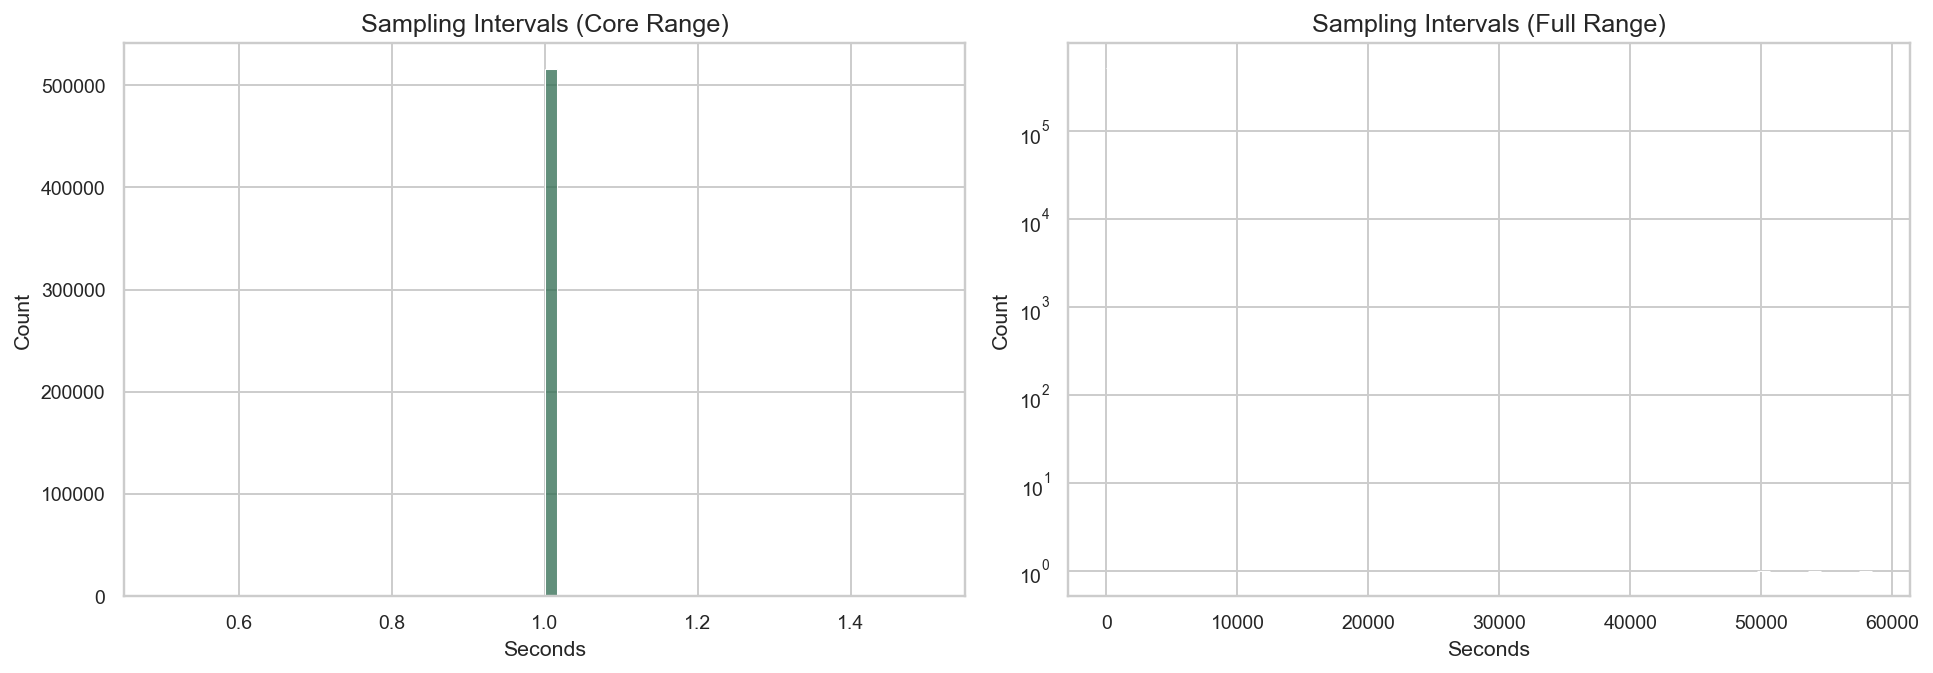
\includegraphics[width=0.8\textwidth]{eda/costa_sampling_intervals.png}
%   \caption{Sampling interval distributions for Costa. Left: histogram zoomed to the 0.6--1.4\,s range, showing a single spike at 1\,s. Right: the complete interval distribution on a log-count axis, exposing the rare gaps above 30\,s.}
%   \label{fig:eda-sampling-costa}
% \end{figure}

\begin{figure}[H]
  \centering
  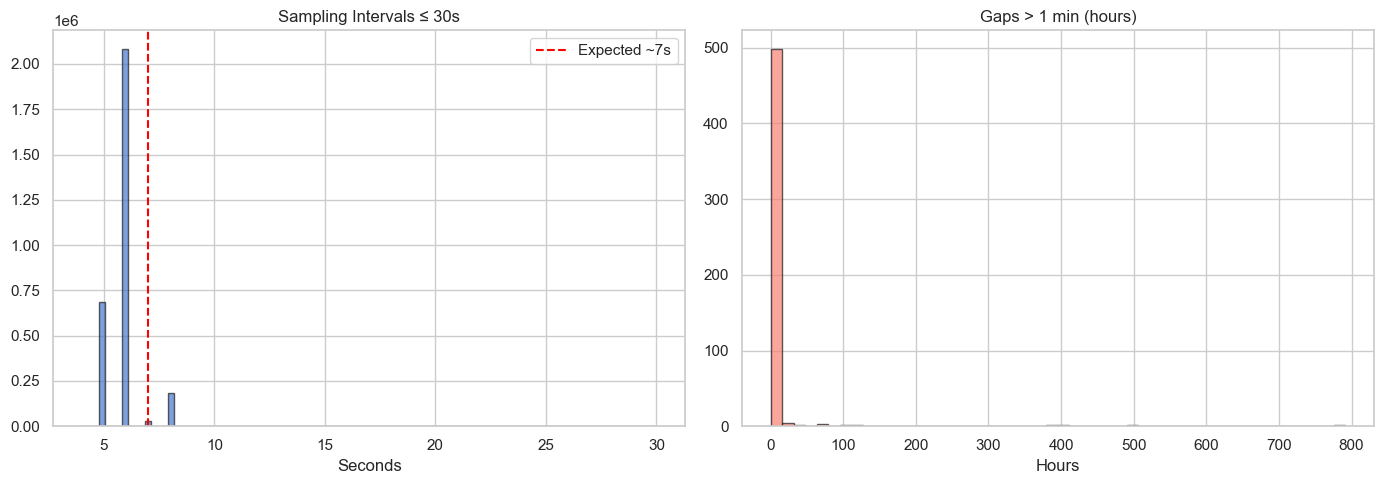
\includegraphics[width=0.8\textwidth]{eda/reunion_sampling_intervals.png}
  \caption{Sampling interval distributions for La~Réunion. Left: intervals up to 30\,s; the dominant mode is 6\,s. Right: frequency of gaps exceeding 1\,minute (x-axis in hours), with 528 such events across the 19-month recording.}
  \label{fig:eda-sampling-reunion}
\end{figure}

\textbf{Missing value analysis.} A field time series can exhibit 3 structurally distinct missingness regimes: Missing Completely At Random (MCAR), where absent values are independent of all observed and unobserved variables; Missing At Random (MAR), where the probability of missingness depends on observed variables; and Missing Not At Random (MNAR), where it depends on the missing value itself. The distinction matters because MCAR and MAR permit principled imputation, while MNAR invalidates it. The null-value share was computed per column and per calendar day, and temporal clustering was assessed to assign each dataset to one of these regimes. For Costa, the irradiance-filtered ingestion frame contains 0 missing values across all 9 channels; the question does not arise. For La~Réunion, Figure~\ref{fig:eda-nulls} shows that missingness in the meteorological channels is sharply concentrated in October--November 2021, converging to near-zero by early 2022. Missingness that is bounded in time, absent from fault-labeled periods, and non-recurrent after the initial deployment window is consistent with an MCAR pattern attributable to sensor commissioning rather than to operating conditions. The tiered imputation in Section~\ref{sec:preprocessing} is therefore applied only to La~Réunion and only to non-fault segments, with a strict prohibition on look-ahead across partition boundaries.

\begin{figure}[H]
  \centering
  \begin{subfigure}[b]{\textwidth}
    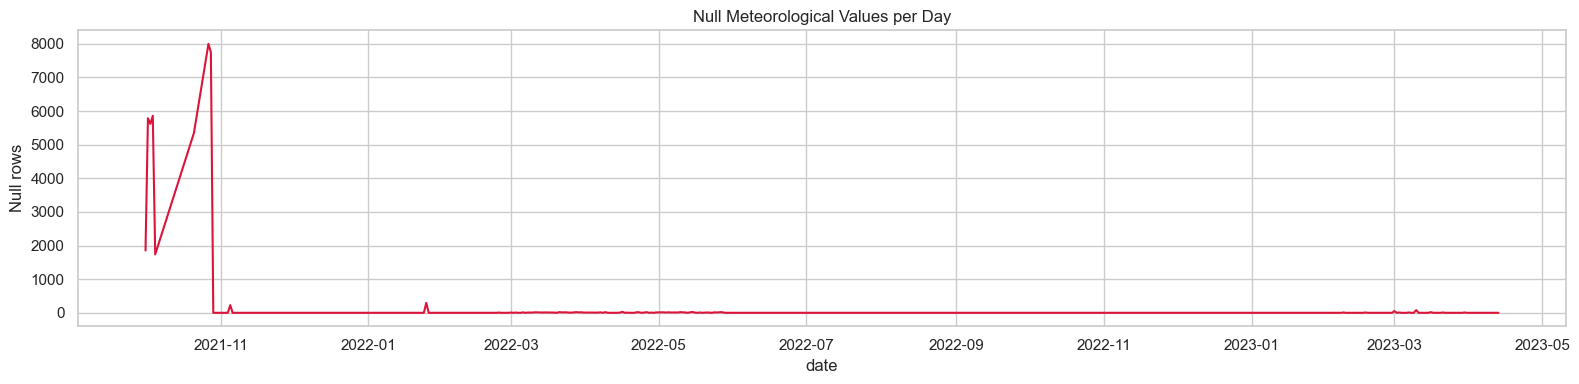
\includegraphics[width=\textwidth]{eda/reunion_null_temporal.png}
    \caption{Meteorological channels.}
  \end{subfigure}
  \vspace{0.4em}
  \begin{subfigure}[b]{\textwidth}
    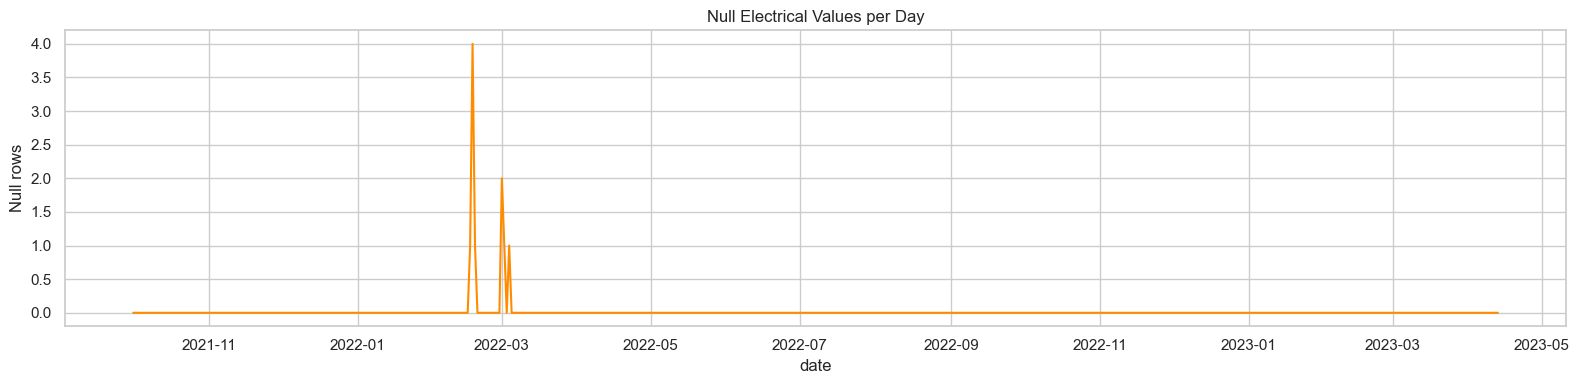
\includegraphics[width=\textwidth]{eda/reunion_null_electrical_temporal.png}
    \caption{Electrical channels.}
  \end{subfigure}
  \caption{Temporal distribution of missing values — La~Réunion.}
  \label{fig:eda-nulls}
\end{figure}

\textbf{Target distribution and fault temporal structure.} The class distribution was examined at 2 levels of granularity: row count and episode count. Figure~\ref{fig:eda-imbalance} shows the row-share versus episode-share for Costa. At the row level, the normal class accounts for 59.9\% and the naturally-occurring shadowing class (label~4) for 35.7\%; the 3 electrically induced fault classes together account for 4.4\%. At the episode level, shadowing occupies 48.9\% of episodes despite its 35.7\% row share, because shadowing episodes are numerous but short (p90 duration $\approx$~91~s), while induced fault episodes are few but long (median $\approx$~590~s for short circuit and open circuit). For La~Réunion, the normal class accounts for 97.2\% of rows, with all fault sub-classes combined below 2.8\%.

\begin{figure}[H]
  \centering
  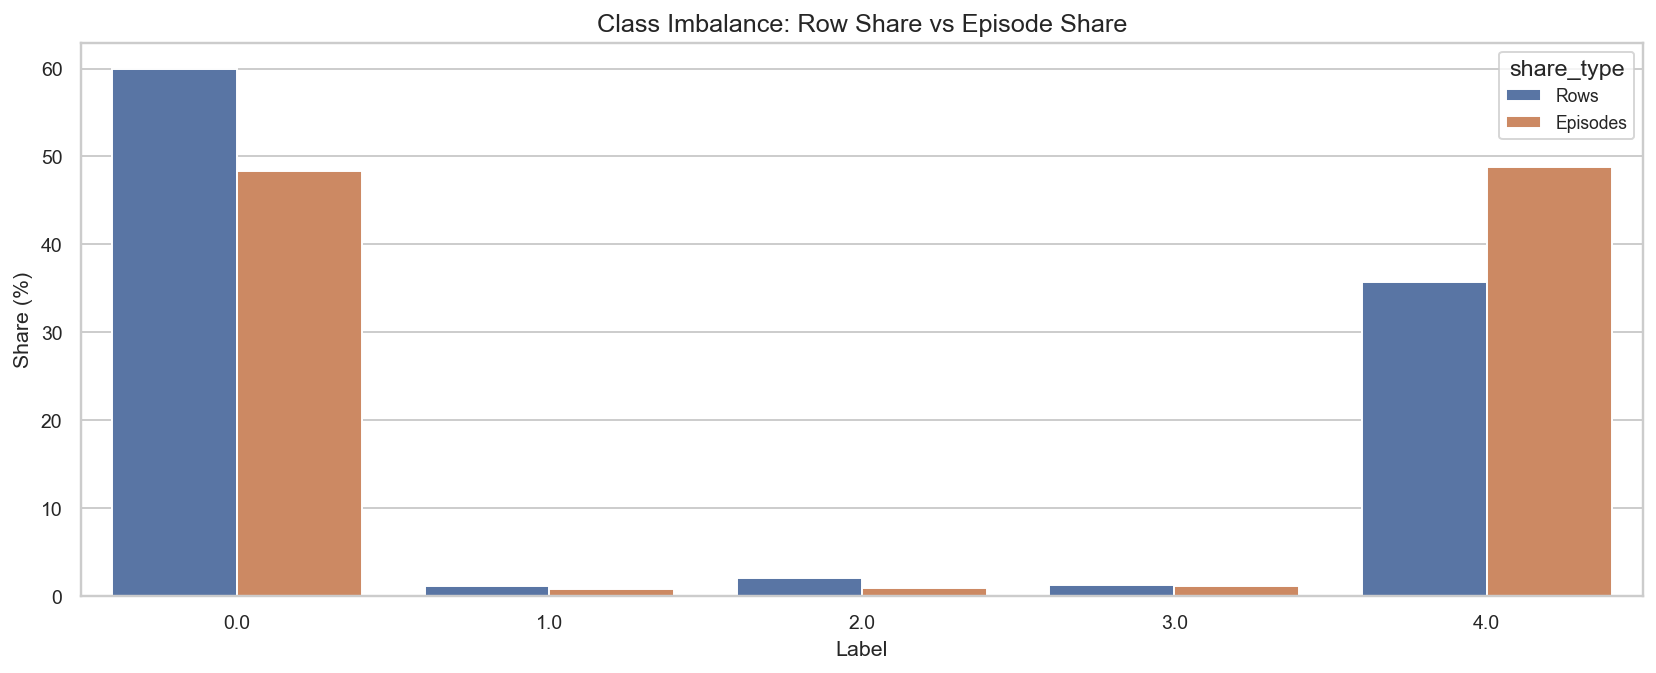
\includegraphics[width=0.80\textwidth]{eda/costa_class_imbalance.png}
  \caption{Class imbalance in Costa at row level versus episode level.}
  \label{fig:eda-imbalance}
\end{figure}

\textbf{Univariate distributions: normal versus fault.} Mann-Whitney U tests were applied in 2 configurations --- binary (normal versus all faults pooled) and per-class (normal versus each fault class individually) --- with Benjamini-Hochberg false discovery rate correction applied to all $p$-values. Figures~\ref{fig:eda-boxplots-costa} and~\ref{fig:eda-boxplots-reunion} show the distributional contrast for the highest-ranked channels. For Costa, all 9 channels produced $p$-values at the numerical floor of zero in both configurations, with FDR correction confirmed for every class combination. The per-class rank-biserial correlations reveal qualitatively distinct signatures: short circuit (label~1) depresses vdc2 toward near-total voltage collapse ($r_{\mathrm{rb}}$ approaching $-1.00$) while elevating idc1; open circuit (label~3) collapses both strings' voltage and current simultaneously (vdc1 at $r_{\mathrm{rb}} = -0.73$); shadowing (label~4) uniformly suppresses current and power in both strings with no corresponding voltage elevation ($r_{\mathrm{rb}}$ between $-0.64$ and $-0.79$). Kruskal-Wallis effect sizes range from $\varepsilon^2 = 0.14$ (vdc2) to $\varepsilon^2 = 0.45$ (idc2), indicating that class membership alone explains up to 45\% of the variance in the DC current channels. For La~Réunion, grid power Pg ($p = 0.15$) and grid current Ig ($p = 0.20$) are not significant under BH-FDR: shading faults reduce irradiance proportionally, so fault-period power values overlap with normal-period values at lower irradiance conditions. These 2 non-significant channels are also those with the highest VIF (Ig = 3,539; Pg = 3,438), so the univariate and collinearity checks converge on the same redundancy.

\begin{figure}[H]
  \centering
  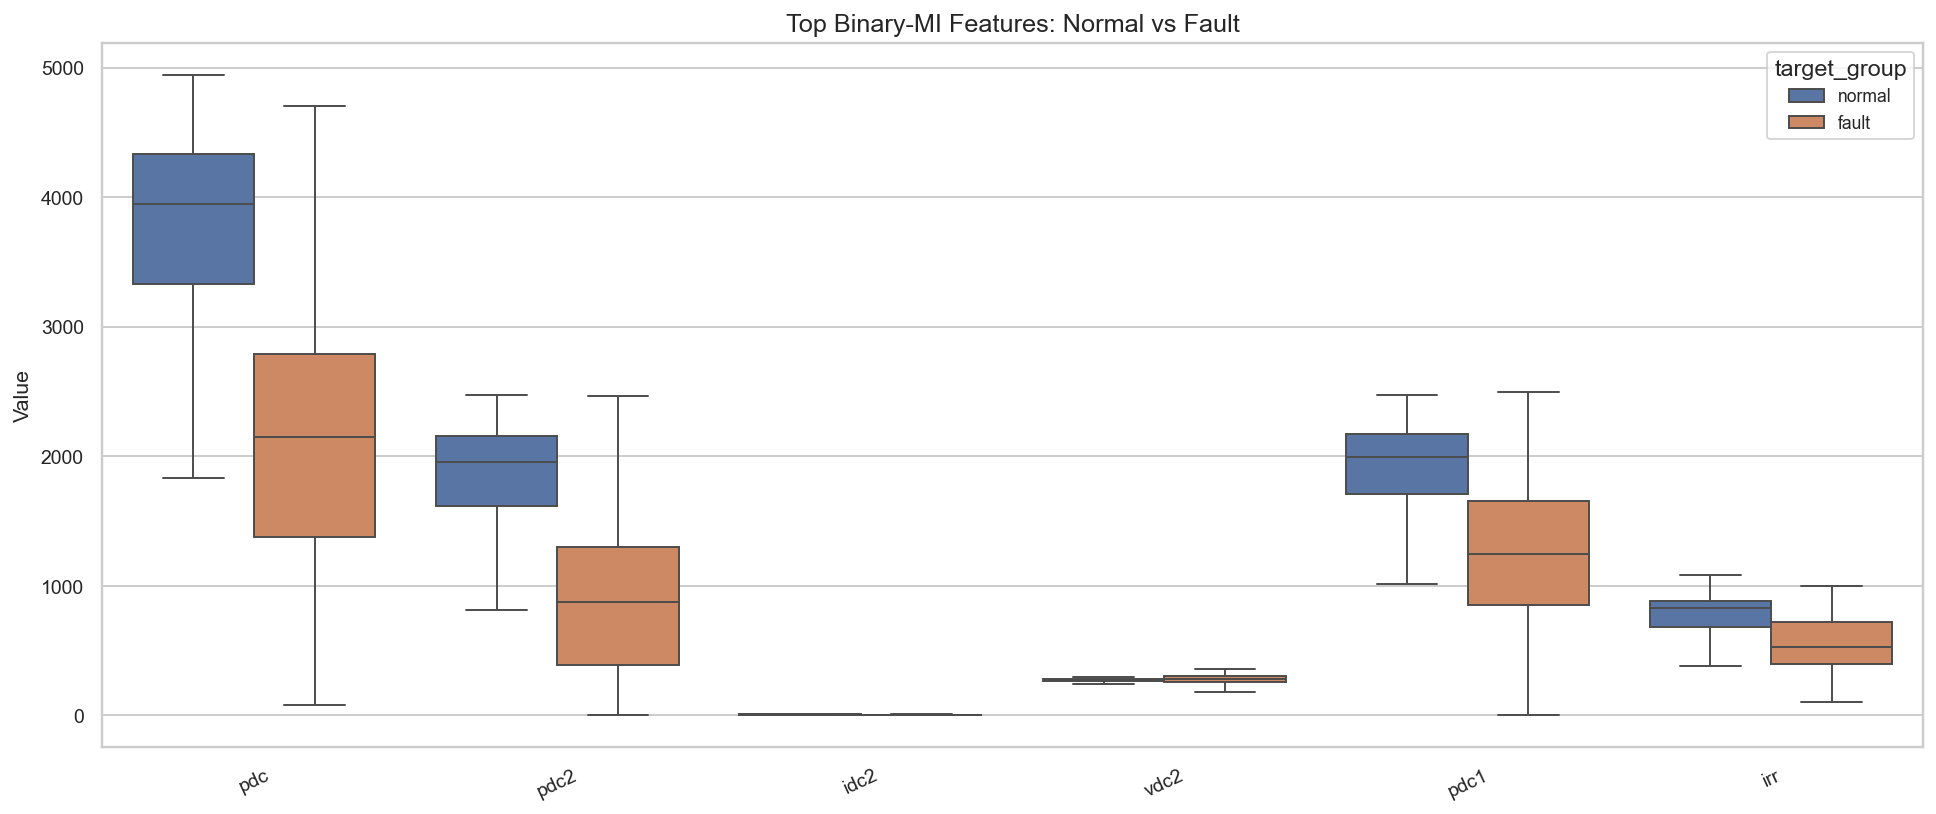
\includegraphics[width=0.8\textwidth]{eda/costa_boxplots.png}
  \caption{Normal versus fault distributional contrast for Costa}
  % : top 5 binary-MI channels. Fault distributions show wider spread and shifted medians. The high-MI power channels exhibit strongly overlapping interquartile ranges at the aggregate level; per-class rank-biserial analysis (discussed in the text) is required to expose the fault-type-specific signatures hidden within this overlap.
  \label{fig:eda-boxplots-costa}
\end{figure}

\begin{figure}[H]
  \centering
  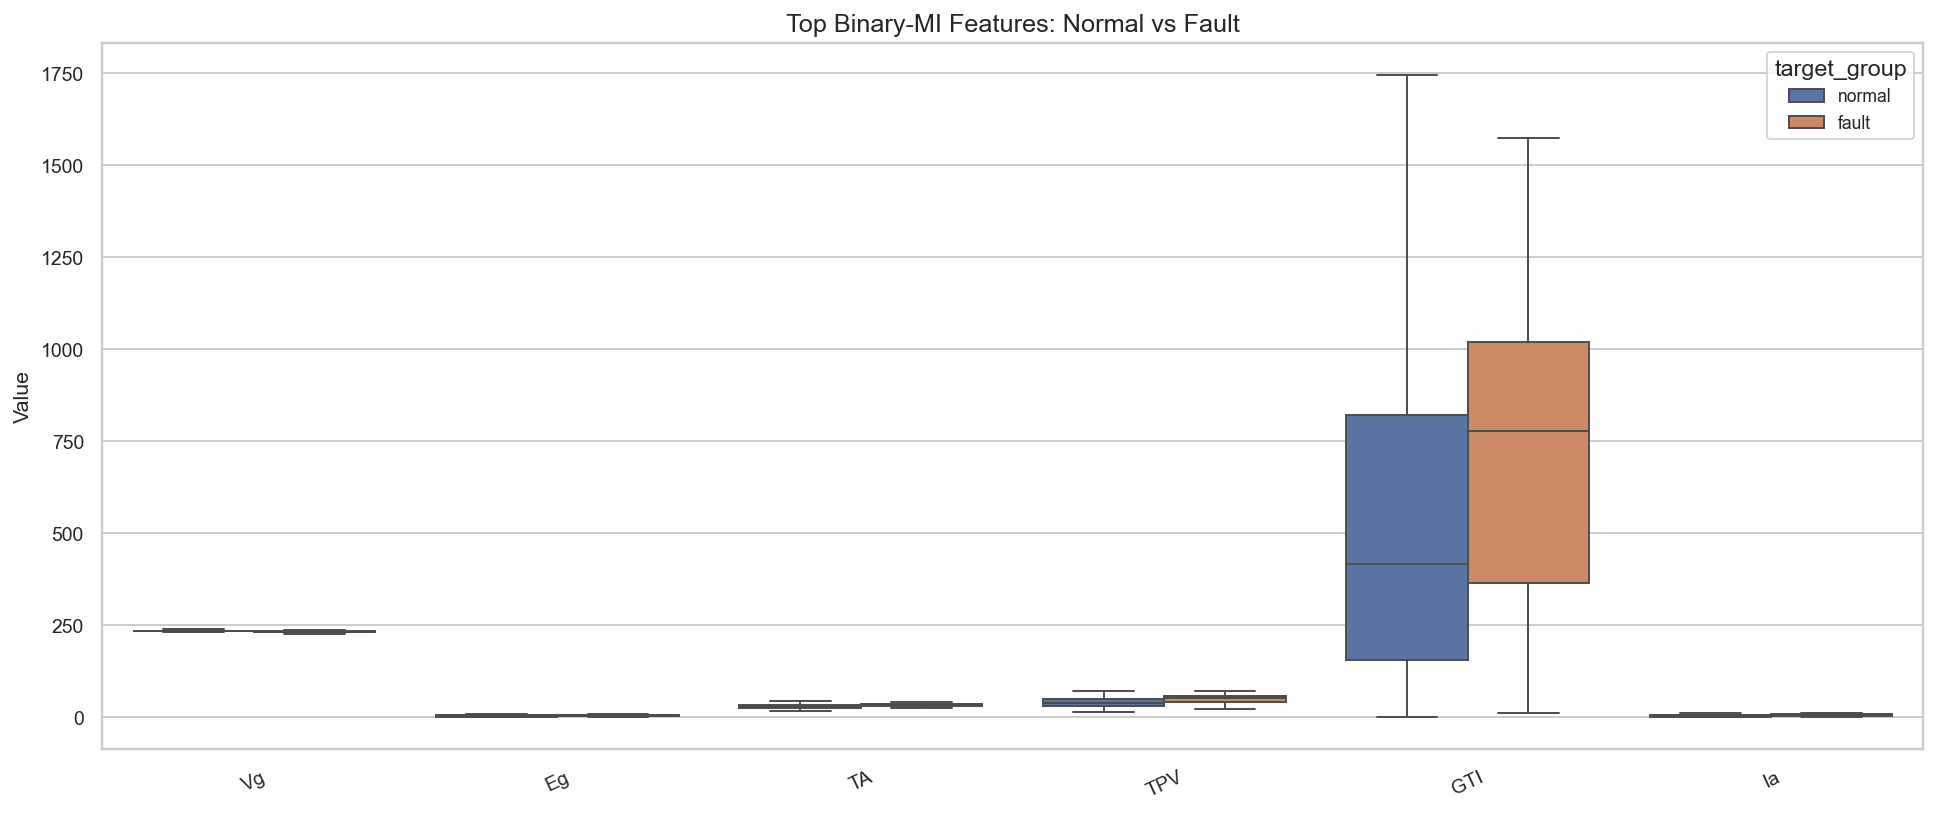
\includegraphics[width=0.8\textwidth]{eda/reunion_boxplots.png}
  \caption{Normal versus fault distributional contrast for La~Réunion}
  % : irradiance-independent channels (Vg, TA, TPV) provide the clearest separation.
  \label{fig:eda-boxplots-reunion}
\end{figure}

\textbf{Irradiance filtering and the production regime.} A 100~W/m$^2$ irradiance floor is applied during Costa ingestion; a GTI-based daytime filter is applied to La~Réunion at the same stage. Rows below these thresholds correspond to night-time or pre-sunrise conditions where all electrical channels are near zero and the class label is uniformly normal by construction. Including these rows would inflate the apparent separability of the normal class from fault classes, creating a spurious detection advantage. All subsequent analysis and modeling operates exclusively on the production regime.

\textbf{Correlation, collinearity, and spurious relationship detection.} Spearman rank correlation was computed in 3 contexts: across all rows, restricted to normal-class rows, and stratified by irradiance quartile within the normal class. Figures~\ref{fig:eda-correlation-heatmap} and~\ref{fig:eda-correlation-regime} show the full normal-class Spearman heatmap and the irradiance-stratified profiles. The normal-class context exposes 2 classes of alias. The first class arises from additive identities: Spearman $\rho$(pdc1, pdc) = 0.999 and $\rho$(pdc2, pdc) = 0.999, empirically confirming $P_{\mathrm{dc}} = P_{\mathrm{dc},1} + P_{\mathrm{dc},2}$; for La~Réunion, $\rho$(Pg, Ig) = 0.9995. The second class arises from the multiplicative physical relationship $P_{\mathrm{dc},s} = V_{\mathrm{dc},s} \cdot I_{\mathrm{dc},s}$ at approximately constant voltage, making per-string current a near-proxy for per-string power ($\rho = 0.976$ for idc1--pdc1). Variance Inflation Factor (VIF) quantifies the regression-based consequence: VIF(\texttt{idc1}) = 187.8 for Costa and VIF(\texttt{Ig}) = 3,539 for La~Réunion. These aliases are the direct targets of the hygiene pruning stage in Section~\ref{sec:feature-engineering}. The irradiance-stratified analysis reveals an additional, non-trivial pattern: while the pdc1--pdc2 correlation remains above 0.95 across all 4 irradiance quartiles, the idc1--idc2 correlation drops to 0.82 in the third quartile (830--885~W/m$^2$) before recovering at peak irradiance. This regime-dependent inter-string divergence is invisible in an aggregate correlation; it is not treated as a data quality artifact but preserved as evidence of non-uniform string behavior under high thermal loading, motivating the per-string imbalance features in Section~\ref{sec:feature-engineering}.

\begin{figure}[H]
  \centering
  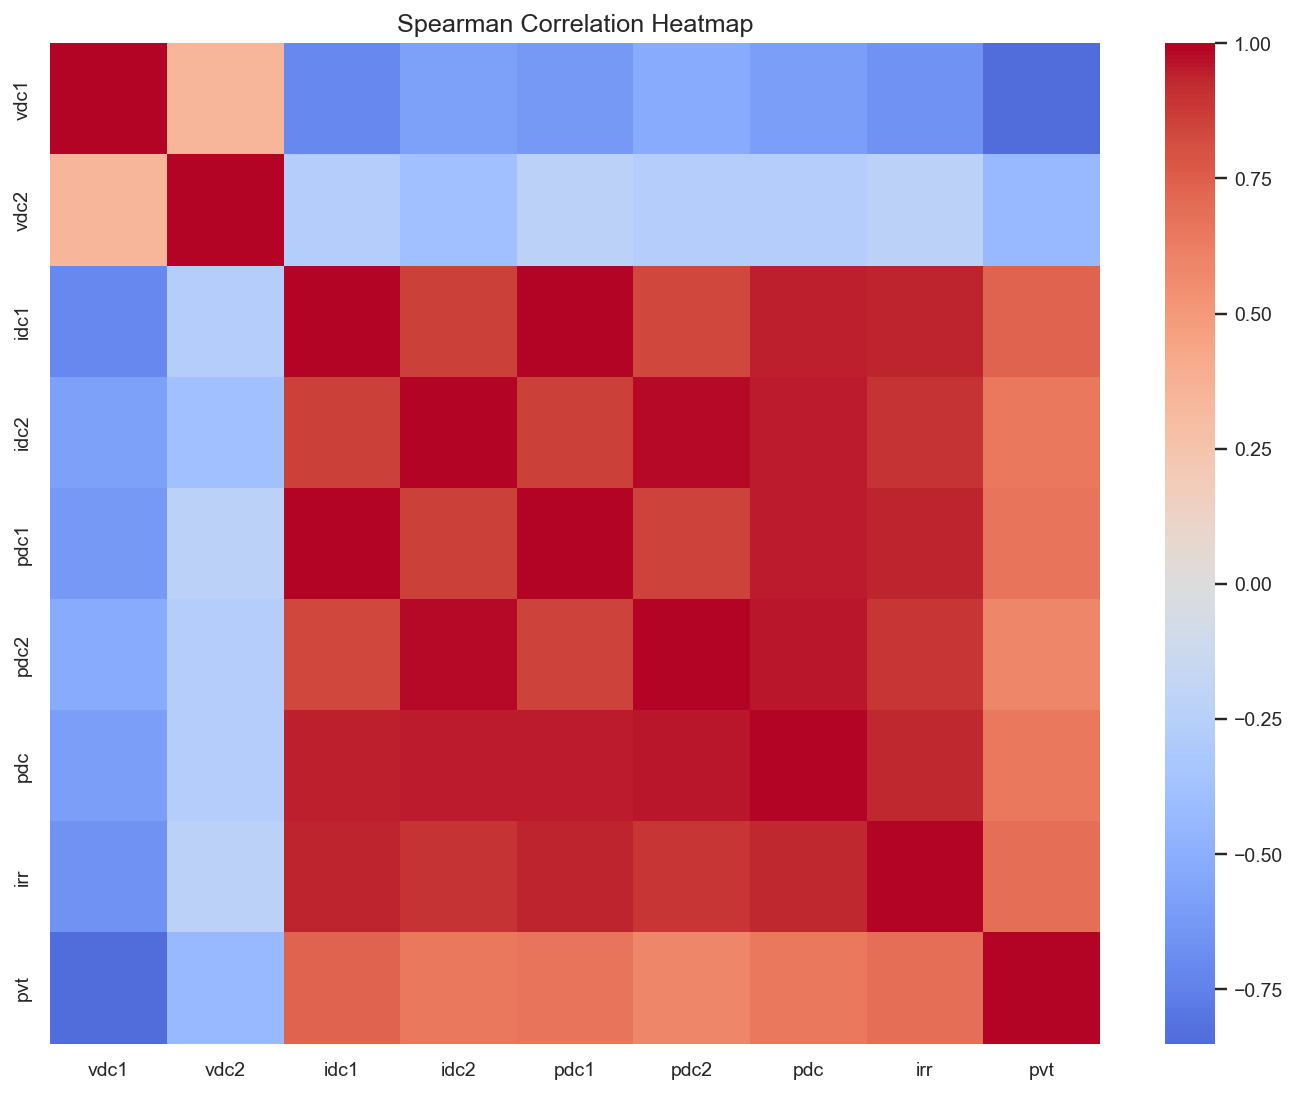
\includegraphics[width=0.8\textwidth]{eda/costa_correlation.png}
  \caption{Spearman correlation analysis for Costa}
  \label{fig:eda-correlation-heatmap}
\end{figure}

\begin{figure}[H]
  \centering
  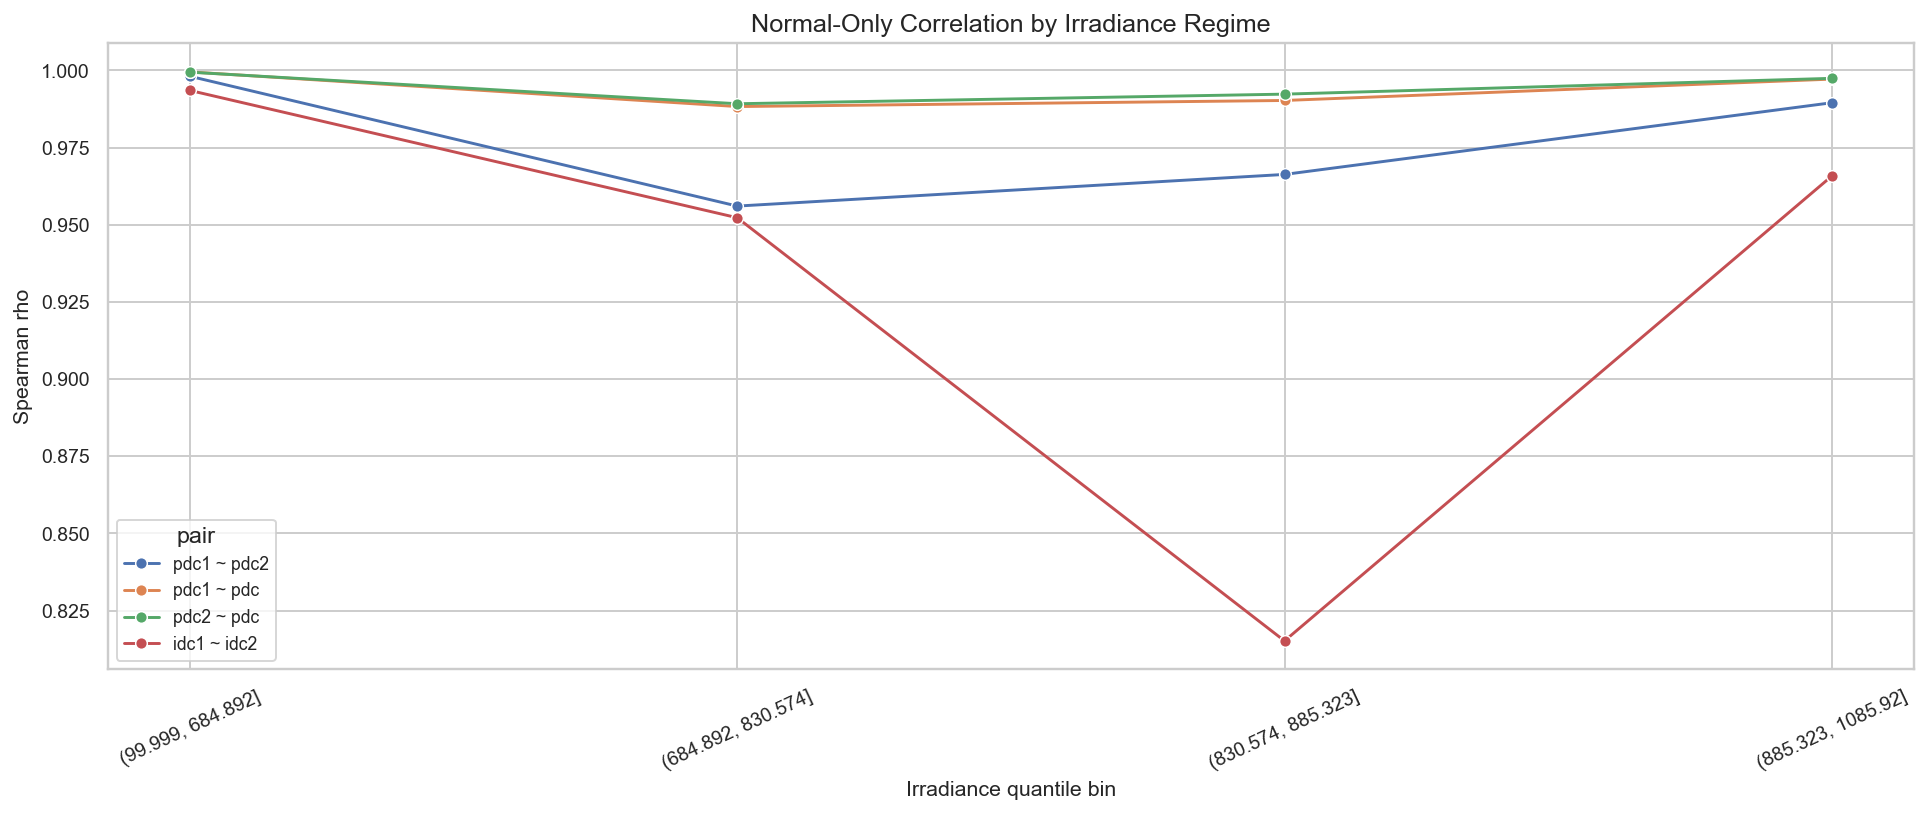
\includegraphics[width=0.8\textwidth]{eda/costa_regime_correlations.png}
  \caption{Spearman correlation analysis for Costa}
  \label{fig:eda-correlation-regime}
\end{figure}

\textbf{Mutual information with target.} Mutual information (MI) was estimated for each raw channel against both the binary fault label and the multi-class label, using a subsampled frame of 100,000 rows. Figure~\ref{fig:eda-mi} shows the comparison for Costa. Multi-class MI is consistently and substantially higher than binary MI across every channel: pdc2 increases from 0.275 to 0.425 bits (a 54\% gap), and idc2 from 0.270 to 0.417 bits. This systematic gap means that feature selection based solely on a binary anomaly label would systematically undervalue channels critical for fault classification. The result motivated the mRMR selection criterion in Section~\ref{sec:feature-engineering} to operate on the multi-class label. For La~Réunion, Vg achieves the highest binary MI (0.026~bits) while Pg achieves only 0.006~bits, providing information-theoretic confirmation of the Mann-Whitney non-significance result: grid power carries negligible discriminative information for shading fault detection.

\begin{figure}[H]
  \centering
  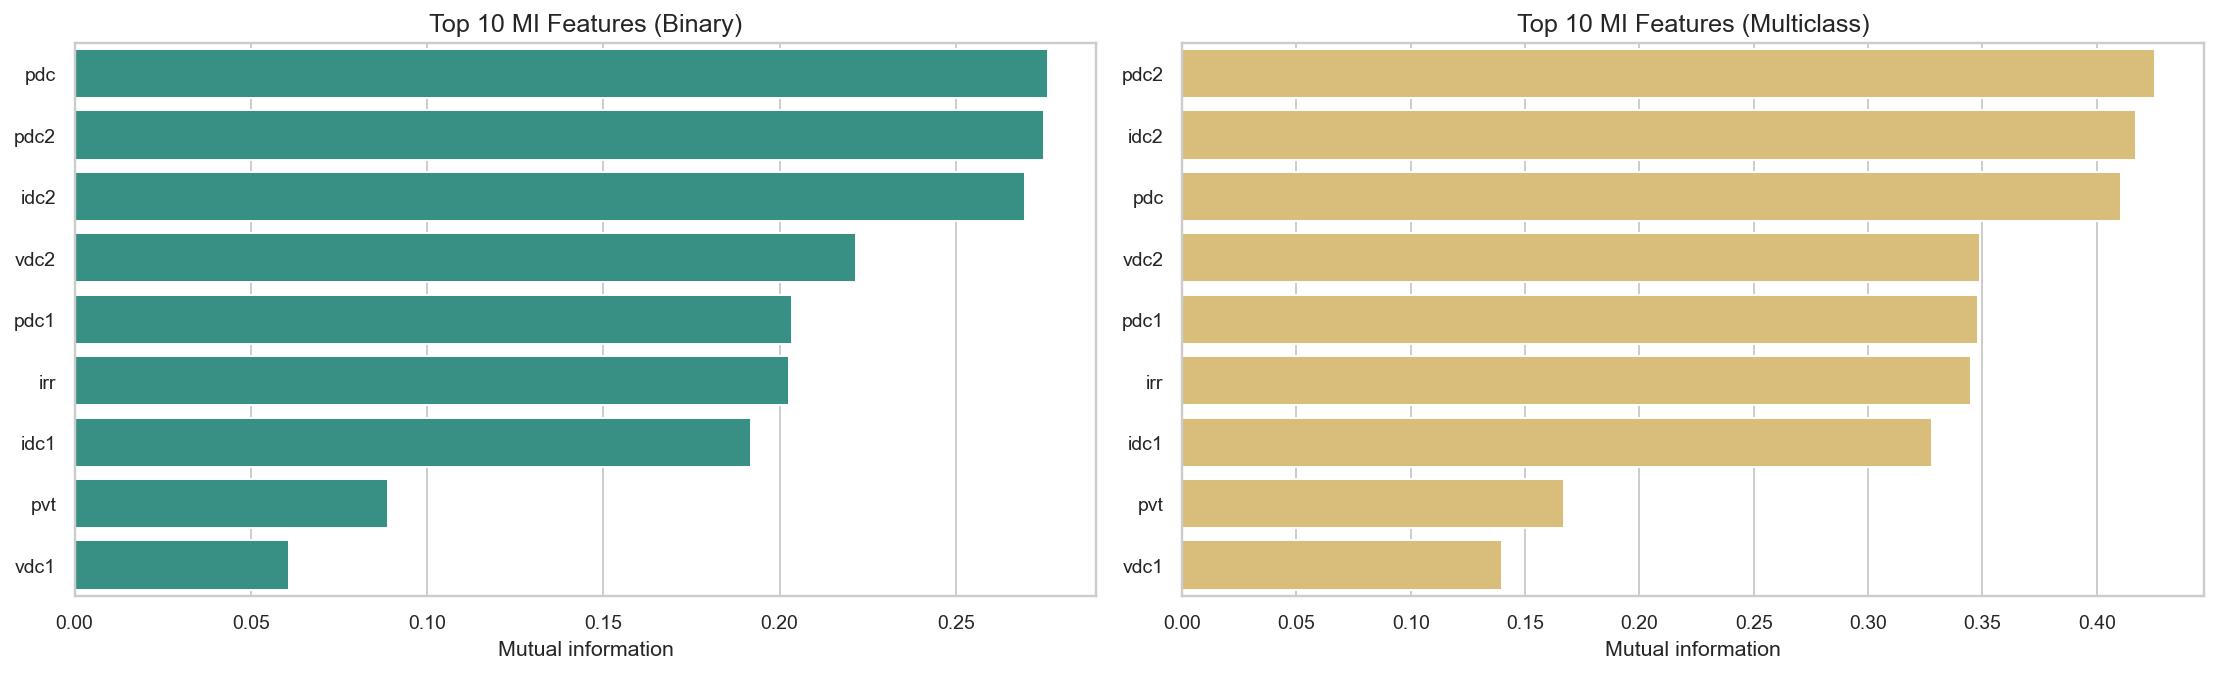
\includegraphics[width=\textwidth]{eda/costa_mutual_info.png}
  \caption{Mutual information against binary (left) and multi-class (right) targets for all Costa channels.}
  \label{fig:eda-mi}
\end{figure}

\textbf{Outlier analysis.} A $3\times\mathrm{IQR}$ criterion was applied exclusively to normal-class rows; bounds were computed from the normal-class IQR and any row falling outside those bounds was flagged. For Costa, the result is strongly channel-asymmetric: idc1, idc2, pdc1, pdc2, pdc, irr, and pvt exhibit 0 outlier rows, while vdc1 yields 1.4\% (4,430 rows). Localizing these vdc1 outliers by date and by hour of day reveals that they are concentrated in the first 3 recording days (2020-04-06 to 2020-04-09) within the 9--12~UTC morning window --- a pattern consistent with system warm-up behavior at the start of the recording rather than with sensor malfunction or any recurring fault. Fault-labeled rows that exceed the same vdc1 bounds are not removed; their extreme voltage values are meaningful fault signatures. This label-aware treatment is the direct specification for the IQR-based preprocessing in Section~\ref{sec:preprocessing}.

\textbf{Stationarity diagnostics.} Augmented Dickey-Fuller (ADF) and KPSS tests were applied to the 5 longest normal-class episodes in each dataset, using a subsampled series to maintain tractable lag selection. The autocorrelation function (ACF) was additionally computed to bound the minimum inter-partition gap needed for temporal independence. Figure~\ref{fig:eda-acf} shows the ACF plots for La~Réunion. The consensus stationarity criterion required ADF rejection of the unit-root null and KPSS non-rejection of the stationarity null simultaneously. Channels including Pg, Ig, GTI, TA, and TPV exhibit ACF values above 0.5 at lag~200 ($\approx$\,23~minutes at 7-second sampling), confirming persistent autocorrelation and non-stationarity within intra-day episodes. This finding has 2 consequences: first, the absolute level of these channels is not a reliable anomaly indicator across episodes recorded at different times of day; second, the minimum inter-partition embargo must span at least 21~minutes to suppress leakage through long rolling features. Both constraints are enforced in Section~\ref{sec:splitting} (21-minute embargo) and Section~\ref{sec:feature-engineering} (first-order temporal derivatives as stationary alternatives to trending raw levels).

\begin{figure}[H]
  \centering
  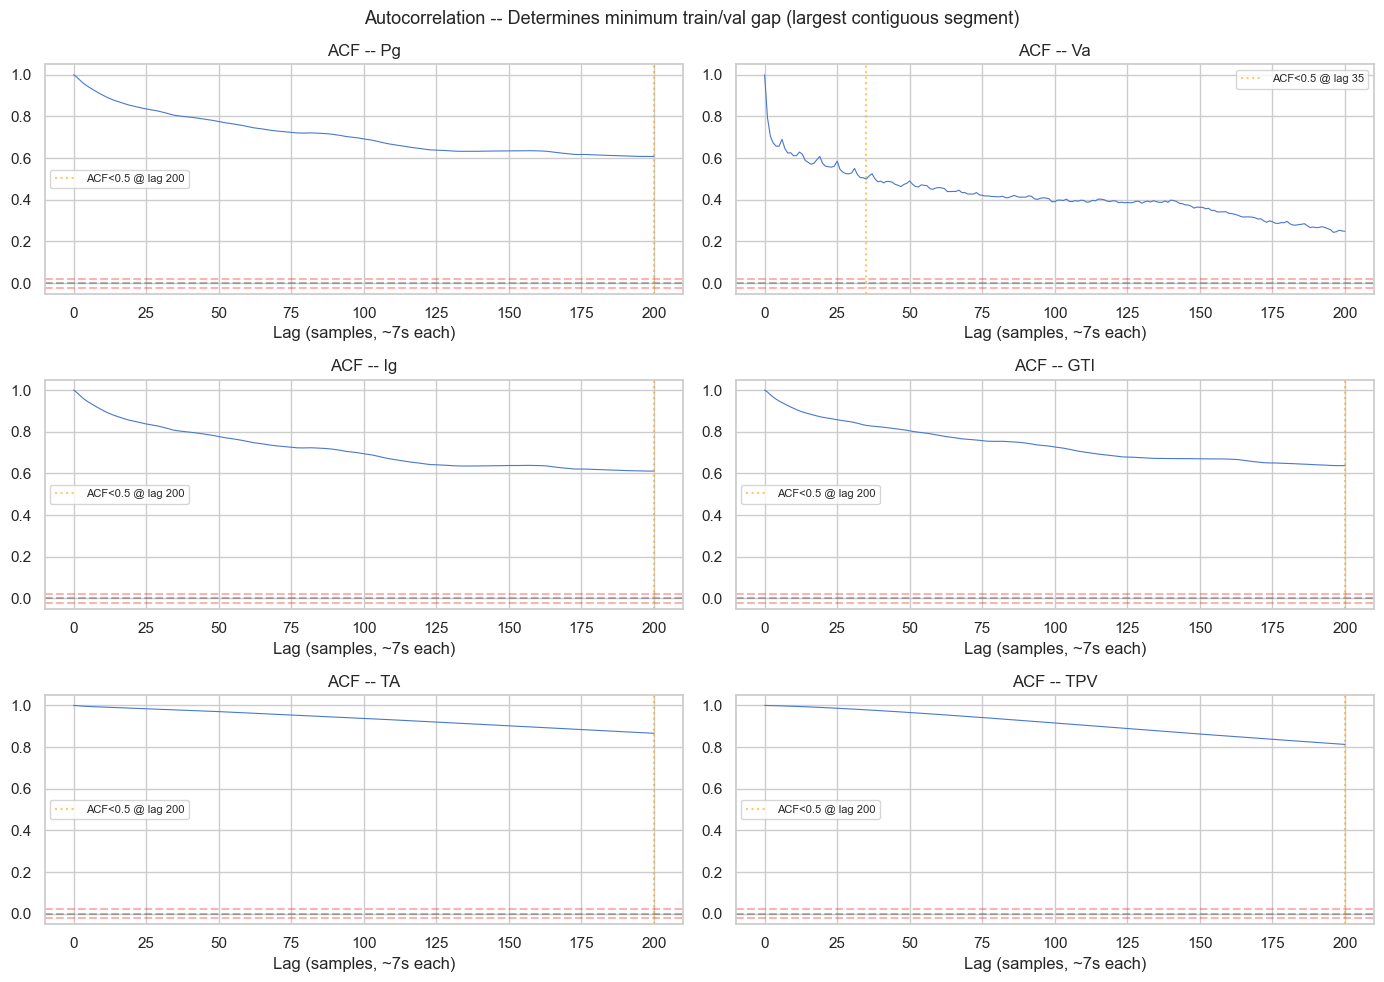
\includegraphics[width=\textwidth]{eda/reunion_autocorrelation.png}
  \caption{Autocorrelation functions for 6 La~Réunion channels computed on the largest contiguous normal-class segment.}
  %  Channels with ACF above 0.5 at lag~200 (orange dashed line, $\approx$\,23~min) are non-stationary within intra-day episodes. This analysis set the minimum train-to-validation embargo at 21~minutes and motivated first-order derivative features as stationary alternatives to the trending raw levels.
  \label{fig:eda-acf}
\end{figure}

\textbf{Sensor health: stuck-at detection and long-term drift.} A rolling variance check was applied across all channels in both datasets: no 30-sample window exhibits zero variance for any electrical channel, confirming that no sensor had frozen at a fixed value. Long-term drift was assessed by computing monthly median values for primary channels over the 19-month La~Réunion recording. PV module temperature (TPV) exhibits a clear seasonal cycle consistent with the Indian Ocean climate; no abrupt calibration jump was detected in any channel. The absence of stuck-at events confirms that no dedicated removal step is required. The smooth seasonal drift is documented as the motivating observation for the drift detection module described in Chapter~\ref{ch:deployment}.


% ────────────────────────────────────────────────────────────
\section{Pipeline Architecture}
\label{sec:pipeline-architecture}
% ────────────────────────────────────────────────────────────
The data pipeline that transforms raw field recordings into the inference-ready representations consumed by every modeling experiment is organized as 5 sequential stages: ingestion, splitting, preprocessing, feature engineering, and model training. This staged organization is a deliberate architectural choice rather than an implementation convenience. A monolithic transformation script would make it impossible to enforce leakage-prevention invariants at a well-defined boundary, to rebuild expensive downstream stages independently when upstream logic changes, or to apply the same pipeline to a new field dataset without touching the transformation code. The staged structure addresses all 3 requirements simultaneously and is the structural foundation of the portability claim: the same pipeline code, parameterized by a site-specific configuration file, produces independent artifact trees for each field dataset with no shared internal state.

The pipeline is constructed as a Directed Acyclic Graph (DAG) of processing stages. Each stage defines formal inputs and outputs, ensuring that downstream processes strictly depend on verified upstream states. This structural abstraction enforces data lineage and prevents the reuse of stale data when upstream logic changes, ensuring end-to-end reproducibility independently of the underlying execution engine. Figure~\ref{fig:pipeline} illustrates the complete pipeline and the role of each stage.
\begin{figure}[H]
  \centering
  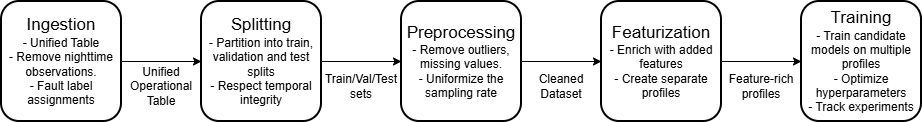
\includegraphics[width=\textwidth]{figures/chap3/pipeline-arch.png}
  \caption{Data pipeline architecture}
  \label{fig:pipeline}
\end{figure}

\begin{itemize}
    \item \textbf{Ingestion} converts raw sensor logs from a given field site into a unified operational table: acquisition streams recorded by heterogeneous systems at different sampling frequencies are joined and aligned, night-time observations are discarded, and the fault condition is assigned to a single shared label column. This conversion is the only stage that carries site-specific format knowledge; every downstream stage receives an identical schema and is fully insulated from the acquisition details of the source system.
    \item \textbf{Splitting} partitions the consolidated table into training, validation, and test sets according to a strict temporal grouping protocol. No sample-level transformation is performed at this stage; splitting is the gate at which evaluation integrity is established, and it must precede all subsequent stages that estimate statistics from the data.
    \item \textbf{Preprocessing} cleans the normal-class rows of the training partition through outlier removal (fault-labeled rows are exempt, as extreme values in those rows are expected fault signatures) and, for sites where the exploratory analysis identifies sustained temporal gaps in the field recording, tiered missing-value imputation, then estimates all cleaning statistics exclusively from that partition and applies them as fixed constants to validation and test.    
    \item \textbf{Feature engineering} transforms cleaned measurements into the representations consumed by the downstream models: named profiles specify which feature families are constructed, and a train-only selection stack eliminates redundant and low-relevance candidates before yielding the final feature matrices. The profile system makes this stage a controlled ablation instrument, isolating the contribution of each feature family across experiments.    
    \item \textbf{Model training} fits each candidate model on the feature-engineered partitions, restricts hyperparameter optimisation strictly to the training and validation partitions, and computes final metrics on the test partition exactly once after the winning configuration has been selected. All configurations, architectural choices, and evaluation results are tracked systematically, ensuring that every reported metric is traceable to a specific architectural state and data partition.
\end{itemize}


% \begin{figure}[H]
% \centering
% 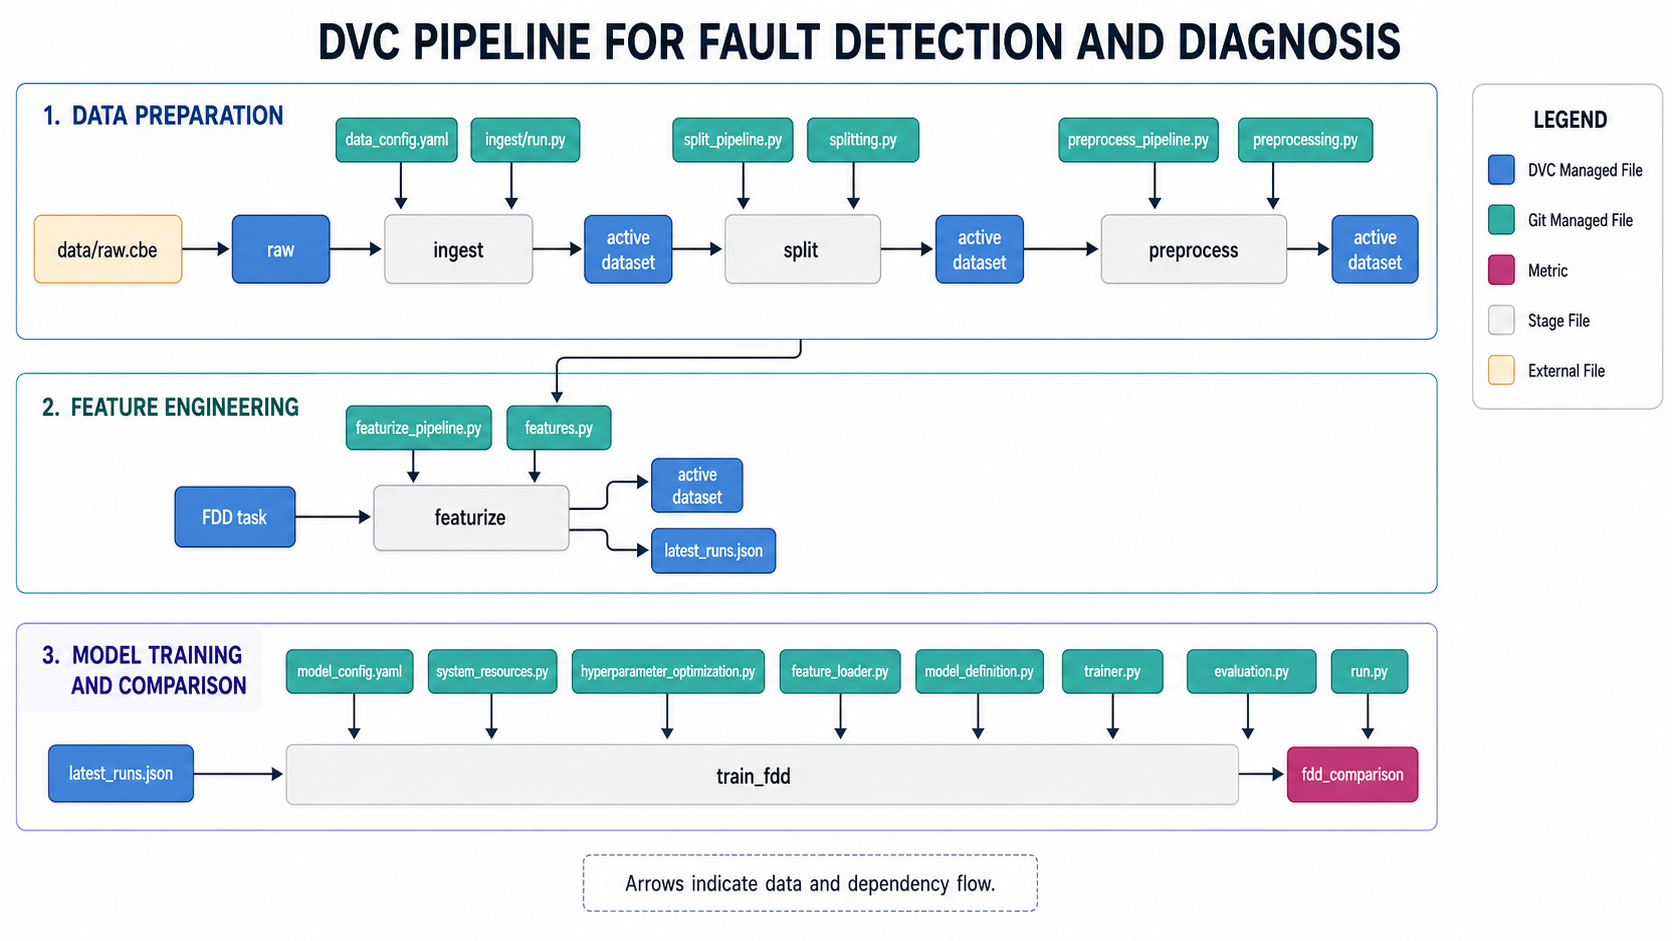
\includegraphics[width=\textwidth]{figures/dvc pipeline.png}
% \caption{Five-stage data pipeline from raw field recordings to model training and edge deployment.}
% \label{fig:pipeline}
% \end{figure}

% ────────────────────────────────────────────────────────────
\section{Conclusion}
% ────────────────────────────────────────────────────────────

This chapter specified the design of the proposed fault detection and diagnosis system for photovoltaic installations, from the high-level system architecture to the data and modeling foundations required for reliable operation on field measurements. Two complementary datasets were selected to support both development and generalization assessment: Costa as the primary multi-fault classification benchmark and La~Réunion as a shading-focused field benchmark under long-term operating variability.

The exploratory audit established the concrete constraints that drive the remainder of the pipeline design. In particular, production-regime filtering prevents artificial class separability from night-time zeros, label-aware cleaning preserves fault signatures while suppressing true sensor glitches, and time dependence is treated as a first-class concern through temporally coherent episode definitions and leakage-preventing partition boundaries. These findings also motivate the feature design philosophy: engineered representations should encode physically meaningful invariants (irradiance normalization, inter-string imbalance, temperature correction, and temporal derivatives) while remaining robust to regime shifts and collinearity.

Finally, the overall pipeline is defined as a staged DAG that separates ingestion, splitting, preprocessing, feature engineering, and model training. This modular structure makes evaluation integrity enforceable at a clear boundary, supports controlled ablations, and enables the same design to be applied consistently across heterogeneous field sites. The next chapter describes how these design requirements are implemented and operationalized in the experimental pipeline.


% \chapter{Data Pipeline Implementation and Experimental Setup}

\section{Introduction}

Following the design phase outlined in the previous chapter, this chapter details the implementation of the data pipeline, specifically the data ingestion, splitting, preprocessing and
feature engineering choices made for the two selected datasets: Costa and La~Réunion, as well as the setup and tools used throughout the development and evaluation of the FDD system.

\section{Tools and Frameworks}
The following tools and libraries were used in the development of the FDD pipeline:
\par\noindent\textbf{Python:} The primary programming language used for data processing, model development, and evaluation.

\par\noindent\textbf{PyTorch:} The deep learning framework used for building and training the machine learning models.

\par\noindent\textbf{Scikit-learn:} A machine learning library used for data preprocessing, feature engineering, and evaluation metrics.

\par\noindent\textbf{Google Colab:} An online platform used for developing and testing the code, as well as for training the models on GPU resources.
\par\noindent\textbf{GitHub:} A version control system used for code management and collaboration.
\par\noindent\textbf{DagsHub:} A platform used for orchestrating and automating the data pipeline, ensuring reproducibility and scalability of the data processing workflow, as well as keeping track of experiments, results and model artifacts.
\par\noindent\textbf{Data Version Control (DVC):} A tool used for versioning datasets and machine learning models, integrated with GitHub for seamless tracking of changes in data and code.
\par\noindent\textbf{MLflow:} A platform used for managing the machine learning lifecycle, including experiment tracking, model versioning, and deployment.


\section{Data Ingestion}
This step involves loading the raw data from the Costa and La~Réunion datasets, then applying a series of transformations to output a unified table ready for the next stage.
These transformations include:
\paragraph{La~Réunion} 
\begin{itemize}
    \item \textbf{Merging:} Read both meteorological and electrical file, then performs a join on the timestamp columns to create a single sorted table with all the features.
    \item \textbf{Column Renaming:} Rename the columns to a unified naming across both datasets.
    \item \textbf{Serializing:} Save the resulting table in a Parquet file and generates a JSON schema manifest. 
\end{itemize}
\paragraph{Costa}
\begin{itemize}
    \item \textbf{Converting:} Convert original raw MAT files to Numpy arrays.
    \item \textbf{Filtering:} Remove negative irradiance values to resolve wrong sensor readings.
    \item \textbf{Timestamp Generation:} Creates a fake synthetic 1 Hz index in microseconds. It anchors the first sample to a specific UTC epoch to align the recorded irradiance curve with local solar noon in Brazil, increasing the time by 1,000,000 microseconds (1 second) per row. 
    \item \textbf{Daytime Trimming:} Filter out nighttime samples by setting a minimum irradiance threshold of 100 W/m².
    \item \textbf{Serializing:} Save the resulting table in a Parquet file and generates a JSON schema manifest.
\end{itemize}

\section{Splitting Protocol}
\label{sec:implementation-splitting}

Because the overall FDD system addresses two distinct operational sub-problems---anomaly detection and fault classification---a single monolithic data split is insufficient. Instead, the pipeline implements a multi-path partitioning algorithm to operationalize essential integrity principles: atomic grouping, temporal ordering, and leakage prevention. Prior to any partitioning, records lacking timestamp or label definitions are dropped as unrecoverable. The partitioning strategy relies on specific structural metadata generated at runtime.

\subsection{Gap-Based Segmentation and Atomic Units}
The first step of the splitting algorithm assigns every row to a contiguous time block. A new \texttt{continuity\_segment\_id} is generated whenever the difference between consecutive timestamps exceeds a 300-second threshold. This 5-minute span is sufficiently large to represent an operational break, such as a night cycle or an extended sensor dropout, effectively separating distinct operational periods. Additionally, a stricter \texttt{episode\_id} is generated that enforces breaks not only at temporal gaps but also at any fault label transition. This ensures that a single segment never contains a mixture of normal and fault conditions. 
For the Costa dataset, \texttt{episode\_id} serves as the indivisible atomic unit for partitioning, ensuring fault episodes are preserved entirely. For the La~Réunion dataset, the broader \texttt{continuity\_segment\_id} is used as the default unit.

\subsection{Task-Specific Allocation Algorithms}
Once atomic units are defined, the pipeline allocates them to training, validation, and test partitions (targeting a 70/15/15 ratio) using structures tailored to the anomaly detection and fault classification tasks.

\paragraph{Hybrid Semi-Supervised Split:}
For the anomaly detection task, the model must map the nominal operational manifold without exposure to labeled fault data. The algorithm selects the chronologically first 70\% of the normal-class segments to form the training partition. The remaining normal segments, alongside all fault-class segments, are split sequentially according to temporal order (50/50) into validation and test partitions. Incorporating faults only in the evaluation sets enforces a strict semi-supervised environment.

\paragraph{Temporal-Stratified Split:}
For the fault classification task, the algorithm executes a temporal-stratified split on each evaluable class independently. It sequences the segments by start time and computes boundary indices that minimize the combined error against the target 70/15/15 ratio for both segment-counts and row-counts, weighting the row-count error at twice the magnitude to select for the learning signal. 
Due to variations in fault distributions, an evaluable-class filter is applied: the Costa processing operates across all five predefined classes (labels 0 through 4), while La~Réunion is restricted to classes exhibiting at least three distinct segments (labels 3.1, 3.2, and 4.0). Classes with insufficient occurrences are restricted to training only, ensuring valid evaluation downstream.

\subsection{Normal-Class Downsampling}
Because normal operating periods vastly outnumber induced fault periods, preserving the complete normal class biases the classification objective. Following the temporal-stratified allocation for the Costa dataset in the fault classification task, the normal class within the training partition is aggressively downsampled to a maximum threshold of 15,000 samples. Crucially, this downsampling extracts a temporal head (the first chronological $N$ rows) rather than a randomized subset. This prevents the fragmentation of local autocorrelation, preserving the structural integrity required for temporal feature generation.

\subsection{Day-Based Chronological Baseline}
To provide a baseline against the class-stratified approach, an independent chronological method is implemented specifically for the Costa dataset. In this pathway, the atomic unit shifts to the \texttt{operating\_day}, with partitions generated as contiguous multi-day blocks. To enforce the temporal embargo specified in the design constraints without discarding entire recording days, the algorithm applies a fraction-based boundary purge: the forward 50\% of the earliest operating day assigned to downstream partitions (validation and test) is dropped. This engineered boundary establishes a chronological gap, preventing look-ahead leakage across overlapping rolling windows.

\section{Preprocessing}
\label{sec:implementation-preprocessing}

The preprocessing stage functions as a minimal cleaning layer between split assignment and feature engineering. Its guiding principle is to preserve the genuine operational signals---both normal and anomalous---required for the downstream tasks while staying as lean as the underlying dataset quality permits. The preprocessing intensity is explicitly calibrated to address the specific structural deficits of each dataset without imposing generic blanket operations. Crucially, all statistics estimated during preprocessing are derived exclusively from the training partition and applied uniformly to the validation and test splits, preventing any possibility of data leakage.

\subsection{Tiered Missing-Value Imputation}
For the Costa dataset, exploration revealed a complete, synthetically indexed 1~Hz timeline devoid of missing values; consequently, imputation routines are disabled for this dataset. Conversely, the La~Réunion dataset exhibits varied temporal continuity gaps extending from seconds to hours. To handle this, a segment-bound, tiered imputation strategy is applied:
\begin{itemize}
    \item \textbf{Short gaps ($\le$ 60 seconds):} Resolved via forward-filling. This assumes transient communication or sensor dropouts where the operational state remains largely static.
    \item \textbf{Medium gaps (60--300 seconds):} Resolved via linear interpolation between bounding observations, relying on the smooth variation of underlying environmental variables.
    \item \textbf{Long gaps ($>$ 300 seconds):} Rows are dropped permanently. Fabricating observations across multi-hour shutdowns or major operational disruptions injects unwarranted artifacts into the modeling pipeline.
\end{itemize}
This imputation is executed strictly on a per-segment basis to prevent bridging distinct operational regimes. Furthermore, a strict override rule is enforced: \emph{if any gap overlaps with a fault-labeled period, those rows are immediately dropped without imputation.} Interpolating across an active fault could artificially synthesize fault signatures, distorting the very deviations the classification model is meant to identify.

\subsection{Outlier Removal}
To address spurious sensor spikes without jeopardizing genuine anomaly detection, a scope-restricted Interquartile Range (IQR) outlier filter is applied. 
The algorithm calculates bounds corresponding to $\text{Q}1 - 3 \times \text{IQR}$ and $\text{Q}3 + 3 \times \text{IQR}$ for primary sensor channels (6 channels for Costa, 9 channels for La~Réunion). A conservative multiplier of 3 ensures only severe sensor malfunctions are flagged.

The bounds are computed exclusively over the normal-class rows of the training partition. Furthermore, the dropping mechanism is applied solely to normal-class segments. Fault-class rows are entirely exempt from outlier rejection because extreme, erratic measurements during those windows represent valid physical fault signatures rather than measurement errors. 

\subsection{Physical Invariant Restoration}
For the Costa dataset, power channels (\texttt{pdc1}, \texttt{pdc2}, \texttt{pdc}) are explicitly derived combinations of raw current and voltage channels. Following the outlier removal phase, it is possible for intermediate states of raw sensors to be dropped, leaving pre-calculated power values disconnected from their constituent variables. To resolve this, all derived power channels are deterministically recomputed from the cleaned primary channels ($P_{\mathrm{dc},s} = V_{\mathrm{dc},s} \cdot I_{\mathrm{dc},s}$). This enforcement maintains the algebraic and physical identities within every row of the final preprocessed dataframe.


% ────────────────────────────────────────────────────────────
\section{Feature Engineering and Profile Ablation}
\label{sec:feature-engineering}
% ────────────────────────────────────────────────────────────

The feature engineering stage transforms cleaned operational measurements into the representations consumed by the downstream models. Two design principles govern its implementation. The first is that features are organized into named profiles, each corresponding to a coherent ablation level that strictly extends its predecessor, enabling a principled comparison of feature representations by contrasting adjacent profile levels. The second is that all selection statistics are estimated exclusively from the training partition, in keeping with the leakage-prevention discipline established in Section~\ref{sec:splitting}.

\subsection{Physics-Informed Features}

The starting point of the profile ladder is a compact set of physics-informed features motivated directly by the exploratory observations of Section~\ref{sec:eda}. These features encode domain knowledge about photovoltaic operation that a purely data-driven model would otherwise have to rediscover from raw observations, and they are constructed to remain numerically stable across the full operating range of the installation.

The first family normalizes power and current channels by the incident irradiance. Under healthy operation, the ratios $P_{\mathrm{dc},s} / G$ and $I_{\mathrm{dc},s} / G$ are approximately constant because irradiance is the dominant driver of both quantities. Normalization collapses the large diurnal amplitude swing present in the raw channels and exposes the fault-related residual that carries the diagnostic signal. The denominator is floored at 1~W/m$^2$ to prevent numerical instability at dawn and dusk.

The second family is the per-string imbalance descriptors. For multi-string installations where each string is individually instrumented, the normalized difference between per-string currents, voltages, and powers provides a sensitive indicator of localized faults that do not manifest in plant-aggregated quantities. Three imbalance features (power imbalance, current imbalance, and voltage imbalance) are computed as normalized pairwise differences and exploit the natural redundancy of the multi-string architecture.

The third family is the temperature-corrected power. The maximum power point of crystalline silicon modules decreases approximately linearly with temperature above the 25\,$^\circ$C standard test condition reference, at a rate given by the module-specific temperature coefficient $\gamma_{P_{\mathrm{max}}}$. The temperature-corrected power divides the observed output by the expected thermal loss factor, and its further normalization by irradiance produces a feature that isolates the fault-related power deviation from the component attributable to ordinary thermal behavior.

The fourth family comprises the first-order temporal derivatives of the primary channels ($\mathrm{d}P/\mathrm{d}t$, $\mathrm{d}V/\mathrm{d}t$, and $\mathrm{d}I/\mathrm{d}t$), computed as discrete differences between consecutive cleaned samples. Rapid transients in current or voltage are characteristic of certain fault types, particularly short circuits and open circuits, and these derivative features expose such transients more clearly than the raw values when the absolute magnitude of the signal is large.

Together, the 4 families yield approximately 17 engineered features after the selection stack described below has pruned the candidate pool. This feature set defines the profile \texttt{plus\_physics}.

\subsection{Profile Ladder}

The named profiles form an additive ablation ladder in which each rung strictly extends the one below it. The 4 profiles evaluated in this thesis are as follows:

\begin{itemize}
    \item \texttt{baseline\_raw}: the cleaned sensor columns produced by preprocessing, with no engineered features. This profile provides the reference level against which the contribution of feature engineering is measured. The hygiene pruning step described below is the only selection applied.
    \item \texttt{plus\_physics}: extends \texttt{baseline\_raw} by adding the 4 physics-informed feature families described above and applying the full hygiene-plus-mRMR selection stack. This is the primary profile used for the headline results in the contribution chapters.
    \item \texttt{plus\_temporal}: extends \texttt{plus\_physics} by adding cyclic encoding of the time of day, representing the hour and minute as sine and cosine projections so that the model receives a continuous, smooth representation of diurnal position without a discontinuity at midnight.
    \item \texttt{plus\_rolling}: extends \texttt{plus\_temporal} by adding causal rolling statistics (rolling mean and rolling standard deviation) over short causal windows, providing the model with a compact summary of recent history that remains strictly within the training partition boundaries.
\end{itemize}

\subsection{Selection Stack}

The candidate feature pool is pruned by a 2-stage train-only selector stack before the final feature set is written to disk. The first stage is hygiene pruning: near-constant columns whose variance falls below a numerical threshold are removed, exact duplicate columns are collapsed, and deterministic algebraic aliases (such as the identity $P_{\mathrm{dc}} = P_{\mathrm{dc}1} + P_{\mathrm{dc}2}$ identified during exploratory analysis) are detected and reduced to a single representative. This stage requires no label information and therefore introduces no leakage risk.

The second stage applies minimum-redundancy maximum-relevance (mRMR) feature selection under the mutual information difference (MID) criterion \citep{peng2005mrmr}, with a target retained pool of 64 features after hygiene. The relevance term scores each candidate by its mutual information with the task label; the redundancy term penalizes mutual information against already-retained features; the greedy selection proceeds until the target size is reached or the pool is exhausted. All mutual information estimates are computed from the training partition only. For large training partitions, estimation is performed on a stratified, group-aware subset of up to 30\,000 rows, which preserves the statistical structure of the label distribution and the temporal grouping while keeping the selection step tractable within the project's computational budget.

% ────────────────────────────────────────────────────────────
\section{Conclusion}
% ────────────────────────────────────────────────────────────

This chapter detailed the technical implementation of the data pipeline, translating the conceptual design requirements into a concrete, reproducible engineering workflow. The end-to-end processing lifecycle, encompassing ingestion, rigorous segmentation, preprocessing, and feature engineering was constructed to strictly safeguard against data leakage and maintain evaluation integrity. By integrating MLOps tools such as DVC for dataset versioning and DagsHub for orchestrating the dependency graph, the pipeline ensures that all intermediate artifacts and final evaluation datasets are perfectly traceable. With the foundational data structures cleansed, standardized, and enriched through ablation profiles, the groundwork is complete. The subsequent chapters will leverage these inference-ready features to formulate, train, and evaluate the specific machine learning architectures selected for the anomaly detection and fault classification models.



% \chapter{Anomaly Detection}

\section{Introduction}
Anomaly detection is the process of distinguishing between normal and anomalous states in a PV system. This chapter introduces the problem, 
then presents the explored models, and finally discusses the experimental results.
% \chapter{Fault Diagnosis}\label{ch:fault-diagnosis}

\section{Introduction}

After an anomalous operating state is detected, the next step in a Fault Detection and Diagnosis (FDD) workflow is to identify the most likely fault type. In practical operation, fault diagnosis supports decision-making by narrowing the set of plausible causes and enabling targeted inspection and corrective actions. In this project, diagnosis is formulated as a supervised multi-class classification task performed on engineered features extracted from the PV system measurements.

Unlike the anomaly detection stage, which aims to separate healthy behavior from abnormal behavior using mostly normal-only training data (Chapter~\ref{ch:anomaly-detection}), the diagnosis stage assumes that labeled fault categories are available for training. The objective is therefore not to produce an anomaly score, but to output a discrete fault class among a predefined set of operating states.

\section{Task Formulation and Methodology}

\paragraph{Problem definition.}
Let $x \in \mathbb{R}^F$ denote a feature vector computed from a time segment of PV electrical and meteorological signals, and let $y \in \{0,\dots,C-1\}$ denote the corresponding fault label among $C$ classes. The diagnosis task consists in learning a classifier $f_\theta$ that maps $x$ to a class probability vector $\hat{p}(y\mid x)$, and predicts the most likely class $\hat{y}=\arg\max_c \hat{p}(c\mid x)$. Because fault classes can be imbalanced in realistic PV logs, the training and evaluation protocol must account for class frequency differences.

\paragraph{Inputs.}
Diagnosis is performed on pre-engineered tabular features rather than on raw time-series windows. Feature computation is executed upstream in the preprocessing and featurization pipeline, and the classification stage consumes the resulting feature tables. This design keeps the diagnosis models lightweight and enables transparent analysis of feature contributions.

\paragraph{Evaluation protocol and metrics.}
The dataset is split into training, validation, and test partitions using the same leakage-aware splitting protocol described in Section~\ref{sec:implementation-splitting}. Model selection is primarily driven by macro-averaged F1-score (macro F1), which assigns equal weight to each class and is therefore sensitive to minority-class performance. For completeness, additional metrics are reported, including overall accuracy, balanced accuracy, macro and weighted precision/recall/F1, and one-vs-rest (OvR) precision--recall AUC values (weighted and per-class).

\section{Shared Experimental Infrastructure}\label{sec:diag-shared-infra}

This section summarizes the shared training and evaluation infrastructure used by all implemented diagnosis models. The common utilities are implemented in the module \texttt{src/modeling/classification/ml/common.py}, and are designed to enforce consistent validation discipline, reproducibility, and comparable reporting across models.

\paragraph{Pipeline overview.}
The diagnosis workflow follows a fixed sequence of stages: data ingestion, split generation, preprocessing, feature extraction, and classifier training. In this chapter, only the classification stage is detailed. The classifier is trained and evaluated exclusively on the engineered feature tables produced by the upstream pipeline.

\paragraph{Feature ingestion and run management.}
Feature tables are loaded through a single entrypoint that resolves the latest (or a specified) feature-generation run for the chosen dataset and feature profile. This mechanism ensures that model runs are traceable to a concrete, versioned feature artifact, and it allows repeatable comparisons across classifiers without re-running feature extraction.

\paragraph{Threading policy.}
To make experimentation efficient and predictable across machines, a resource-aware threading policy is applied. The available CPU budget is detected automatically, one core is reserved for the operating system, and the remaining threads are split between parallel hyperparameter optimization trials and per-trial model training threads. Command-line overrides allow the user to bound the total thread usage and the number of parallel optimization jobs.

\paragraph{Label encoding.}
Fault labels are encoded into contiguous integer identifiers $\{0,\dots,C-1\}$ using a fitted label encoder. The encoder is trained on the training labels and then applied unchanged to validation and test partitions. It is serialized alongside the model artifact to ensure that inference uses the same class mapping as training.

\paragraph{Hyperparameter optimization (HPO) and validation modes.}
All implemented diagnosis models support automatic hyperparameter optimization through a unified interface. Two validation modes are available. The default mode uses a classical holdout protocol in which each trial is fitted on the training partition and scored on the validation partition using macro F1. An alternative mode performs a per-class, segment-aware temporal cross-validation in which folds follow an expanding-window structure. This second mode provides a stronger guard against temporal leakage when fault segments exhibit time-dependent structure.

\paragraph{Probability calibration.}
In addition to maximizing classification accuracy, reliable probability estimates are important for downstream decision-making (e.g., confidence-based alerting and operator interfaces). Therefore, an optional probability calibration stage is enabled by default. After a base classifier is fitted on the training partition, a calibration model is fitted on the validation partition using sigmoid calibration (Platt scaling). Both uncalibrated and calibrated probability outputs are evaluated on the test set. Calibration quality is summarized with metrics such as log loss, a multi-class Brier score, and bin-based calibration errors including the Expected Calibration Error (ECE) and Maximum Calibration Error (MCE).

\paragraph{Leakage checks.}
Before and after training, automated checks are executed to detect common leakage failure modes. In particular, an exact-duplicate overlap check verifies that identical feature rows do not appear across training and validation partitions, and a leakage report is produced on the test partition unless explicitly skipped. These controls complement the splitting protocol by providing empirical evidence that partition boundaries are respected.

\paragraph{Reporting artifacts.}
To facilitate interpretability and comparison, all models produce a consistent reporting suite. This includes a confusion matrix (raw counts and normalized), OvR precision--recall curves per class, a predicted-class distribution plot, and reliability diagnostics when calibration is enabled. For tree-based models that expose feature importance scores, the top-ranked features are also reported to support qualitative analysis of which engineered variables drive the diagnosis decisions.

\section{Model Lineup and Results}\label{sec:diag-model-lineup}

This section presents the classification models implemented for fault diagnosis. All models operate on the same engineered feature representation and are trained and evaluated under the shared infrastructure described in Section~\ref{sec:diag-shared-infra}.

\begin{table}[H]
\centering
\caption{Summary of implemented diagnosis models and their shared training protocol. HPO: Hyperparameter Optimization.}\label{tab:diag-model-summary}
\begin{tabular}{lccc}
\toprule
\textbf{Model} & \textbf{Family} & \textbf{Class balancing} & \textbf{Calibration}\\
\midrule
LightGBM      & Gradient-boosted trees & Balanced class weights & Sigmoid on validation\\
CatBoost      & Gradient-boosted trees & Balanced class weights & Sigmoid on validation\\
ExtraTrees    & Randomized tree ensemble & Balanced class weights & Sigmoid on validation\\
\bottomrule
\end{tabular}
\end{table}

\subsection{LightGBM Classifier}

LightGBM is a gradient-boosting framework that builds an ensemble of decision trees sequentially, where each new tree focuses on correcting the errors made by the current ensemble. In the diagnosis setting, the model learns non-linear decision boundaries over engineered features and can capture complex interactions between electrical indicators and contextual variables. LightGBM is selected as the default classifier because it provides a strong accuracy--efficiency trade-off on tabular data and scales well during hyperparameter search.

To mitigate class imbalance, the training procedure applies automatic class weighting so that minority fault classes receive proportionally higher penalty when misclassified. Hyperparameters such as the learning rate, number of boosting rounds, and tree complexity are tuned using the shared HPO protocol. When probability calibration is enabled, a sigmoid calibrator is fitted on validation predictions to improve the alignment between predicted confidence and empirical correctness.

\paragraph{Results}
% Intentionally left blank (to be filled with experimental results and analysis).

\subsection{CatBoost Classifier}

CatBoost is another gradient-boosting method that uses symmetric trees and an ordered boosting strategy designed to reduce prediction shift during training. Although CatBoost is particularly known for robust handling of categorical features, it also performs competitively on fully numerical feature sets and offers stable optimization behavior. In this project, CatBoost is implemented as an alternative to LightGBM within the same training harness.

The model is tuned with the same primary objective (macro F1) and the same validation modes. Class imbalance is handled through the algorithm's native balanced class-weighting mechanism. When enabled, the same sigmoid calibration stage is applied to CatBoost probability outputs using validation data.

\paragraph{Results}
% Intentionally left blank (to be filled with experimental results and analysis).

\subsection{ExtraTrees Classifier}

ExtraTrees (Extremely Randomized Trees) is an ensemble method that averages the predictions of many decision trees built with strong randomization. In contrast to boosting, trees in ExtraTrees are trained largely independently, and randomness is injected by selecting split thresholds at random. This often yields robust performance with limited tuning effort, and it provides a useful non-boosting baseline for engineered-feature classification.

In the implemented pipeline, the number of trees, depth limits, split constraints, and feature subsampling strategy are tuned under the shared HPO protocol. Class imbalance is handled via balanced class weights. Probability calibration, when enabled, follows the same validation-based sigmoid calibration procedure.

\paragraph{Results}
% Intentionally left blank (to be filled with experimental results and analysis).


\chapter{Implementation and Evaluation of the Anomaly Detection and Fault Diagnosis Pipeline}
\label{ch:implementation}

\section{Introduction}
This chapter details the implementation of the anomaly detection and fault diagnosis methods explored during this project. It covers the model architectures, training procedure and results
obtained from the evaluation on the Costa dataset.

\section{Tools and Experimental Setup}
\subsection{Software and Libraries}
The implementation relies on a small set of libraries and services, grouped by their role in the end-to-end pipeline.

\subsubsection{ML/DL core}
\par\noindent\textbf{Python:} The primary programming language used for data processing, model development, and evaluation.
\par\noindent\textbf{PyTorch:} The deep learning framework used for implementing and training the neural models.
\par\noindent\textbf{Scikit-learn:} Used for preprocessing, classical baselines, and evaluation metrics.
\par\noindent\textbf{SciPy:} Scientific computing utilities used for numerical routines and statistical operations required by parts of the pipeline.
\par\noindent\textbf{Optuna:} Hyperparameter optimization framework used to tune model configurations under a shared HPO protocol.

\subsubsection{Data engineering and visualisation}
\par\noindent\textbf{Polars:} A high-performance DataFrame library used for efficient tabular data transformations in the preprocessing and feature engineering stages.
\par\noindent\textbf{Matplotlib:} Used to generate diagnostic plots and result figures (e.g., curves and confusion matrices).

\subsubsection{Experiment tracking and reproducibility}
\par\noindent\textbf{GitHub:} Used for version control and collaborative code management.
\par\noindent\textbf{Data Version Control (DVC):} Used to version datasets and large artifacts, and to encode the multi-stage pipeline as reproducible dependency graphs.
\par\noindent\textbf{MLflow:} Free software used for experiment tracking, metrics logging, and model versioning.
\par\noindent\textbf{DagsHub:} Used as a centralized platform for hosting the DVC remote and the MLflow tracking server, enabling traceability of runs and artifacts.
\par\noindent\textbf{Google Colab:} Used as a managed GPU-backed execution environment for deep learning training and hyperparameter search.

\subsection{Experimental Setup}\label{sec:implementation-experimental-setup}
This section summarizes the software stack and execution environment used to implement and evaluate the proposed Fault Detection and Diagnosis (FDD) pipeline. The goal is to ensure that the reported results can be reproduced from a versioned codebase, a traceable dataset state, and a documented configuration.

\paragraph{Codebase and execution contract.}
All experiments are implemented as a Python (\(\geq 3.11\)) monorepository, where each pipeline stage is exposed through a module entry point executed with a unified invocation pattern (e.g., \texttt{uv run python -m src.data.ingestion}). The \texttt{uv} build system is used as the only package and environment manager, ensuring consistent dependency resolution across local and cloud execution.

\paragraph{Configuration management.}
To minimize implicit assumptions and to enable systematic comparisons, all data and model decisions are externalized into YAML configuration files. The data configuration defines the active dataset, split policy, preprocessing options, and feature profiles, while the model configuration defines the active model lineup, hyperparameter optimization (HPO) settings, and detector-specific post-processing (e.g., anomaly threshold calibration). When multiple configuration scopes apply, parameters are resolved through a deterministic hierarchy (global defaults, dataset overrides, task directives, then profile overrides), which prevents silent overrides and simplifies run auditing.

\paragraph{Data versioning and pipeline reproducibility.}
Large artifacts (raw data, processed tables, and selected model checkpoints) are managed with Data Version Control (DVC). The end-to-end workflow is encoded as a multi-stage DVC pipeline (ingestion, splitting, preprocessing, featurization, and training), such that intermediate artifacts are regenerated from their upstream dependencies and tracked through content hashes. The DVC remote storage is hosted on DagsHub, while Git stores the lightweight \texttt{.dvc} pointers and the pipeline definition. This separation keeps the repository manageable while preserving traceability between the reported metrics and the exact data state that produced them.

\paragraph{Compute environments and execution discipline.}
Two execution environments are used depending on workload characteristics. CPU-oriented stages, including ingestion, exploratory analysis, and the classical machine learning baselines, are executed on a local machine. Deep learning training and HPO are executed on Google Colab with GPU acceleration (typically NVIDIA T4 or A100). In Colab sessions, a persistent Google Drive workspace is mounted and used as an artifacts root directory, so that Optuna studies, checkpoints, metrics, and plots survive runtime disconnections. This split avoids wasting GPU resources on CPU-bound data manipulation and focuses accelerated compute on the training loops that benefit from it.

\paragraph{Hyperparameter optimization protocol.}
% Model selection is conducted with Optuna using the Tree-structured Parzen Estimator (TPE) sampler. Classical models are tuned with fixed trial budgets, where each trial is fast and therefore pruning is not required. Deep learning models use the same Optuna interface but can additionally enable early stopping and pruning strategies, because training a single trial can span multiple epochs. For all tasks, the validation partition is the only split used for HPO decisions (metric optimization and threshold selection), while the test partition is reserved for final reporting.
Each model evaluated in this work exposes a set of parameters that govern its capacity and training dynamics (learning rate, regularization coefficients, architectural dimensions) but that training itself cannot determine. These must be selected through a separate optimization process driven by a held-out validation signal. A systematic, automated search is necessary: the number of candidate configurations is too large for manual exploration, and deep learning models in particular carry non-trivial trial costs that penalize exhaustive strategies.

Two complementary optimization strategies are employed depending on the model family. For most classical and deep learning models, optimization is performed using Optuna \citep{akiba2019optuna} with the Tree-structured Parzen Estimator (TPE) sampler. Rather than enumerating a predefined grid of configurations as grid search does \citep{bergstra2012random}, or evolving a population of candidates as genetic algorithms require, TPE builds a probabilistic model of the objective from the history of completed trials and focuses subsequent sampling on the regions associated with good outcomes. This sequential, model-guided search reaches competitive configurations in far fewer trials than either exhaustive or population-based alternatives, which is decisive when individual trials involve full training runs of deep architectures.

The second strategy is the Good-point-set Vectorised Snow Ablation Optimiser (GVSAO), a population-based metaheuristic derived from the snow ablation algorithm \citep{GTBADGVSAOTransformerBiLSTMbasedTimeseries2026}. GVSAO initialises a population of candidate solutions using a good-point-set method that ensures uniform coverage of the search space from the first generation. Each candidate is evaluated on the objective, and the population is refined over successive generations through dual-population dynamics that balance exploration and exploitation: one sub-population performs local refinement around high-quality solutions while the other maintains diversity by searching less-visited regions. Adaptive melting factors modulate the intensity of this competition across generations, and periodic oscillation mutations inject controlled randomness to prevent premature convergence. Unlike TPE, which builds a probabilistic model of the objective surface from trial history, GVSAO directly navigates the parameter space through coordinated agent movement, making it suitable when the evaluation budget is small and the overhead of maintaining a surrogate model would outweigh its benefit.

Each HPO study runs on the fixed original train/val split and completes before the K-fold cross-validation begins, so the winning configuration is fixed for all folds. The test partition is invisible throughout. The optimization objective is the validation macro per-class PR-AUC for anomaly detection and the validation macro F1 for fault classification, consistent with the headline metrics of Section~\ref{sec:evaluation-methodology}. Among configurations whose scores fall within one standard deviation of each other, the simpler configuration is preferred as a tiebreaker.

The pruning strategy is adapted to trial cost. For classical ML models, no pruner is applied: trials are inexpensive and no intermediate epoch-level signal is available. For deep learning models, a Median pruner is added: a trial is terminated when its intermediate validation score falls below the median of all completed trials at the same epoch, after a warmup period during which pruning is suspended. Within-trial early stopping patience scales with the trial epoch budget, preventing premature termination on short trial budgets.


\paragraph{Experiment tracking and artifacts.}
All runs are tracked with MLflow and logged to a centralized DagsHub tracking server. Each run records the active dataset and split identifier, the selected feature profile, the final HPO parameters, and the computed validation and test metrics. In addition, lightweight artifacts are stored alongside metrics, including serialized preprocessing objects (e.g., scalers), model files (\texttt{.joblib} for classical models and checkpoints for deep learning), and diagnostic figures such as PR curves, score histograms, and confusion matrices. This tracking discipline supports direct comparison across the anomaly detection and fault classification experiments.



\chapter{Anomaly Detection}

\section{Introduction}
Anomaly detection is the process of distinguishing between normal and anomalous states in a PV system. This chapter introduces the problem, 
then presents the explored models, and finally discusses the experimental results.


\chapter{Fault Diagnosis}\label{ch:fault-diagnosis}

\section{Introduction}

After an anomalous operating state is detected, the next step in a Fault Detection and Diagnosis (FDD) workflow is to identify the most likely fault type. In practical operation, fault diagnosis supports decision-making by narrowing the set of plausible causes and enabling targeted inspection and corrective actions. In this project, diagnosis is formulated as a supervised multi-class classification task performed on engineered features extracted from the PV system measurements.

Unlike the anomaly detection stage, which aims to separate healthy behavior from abnormal behavior using mostly normal-only training data (Chapter~\ref{ch:anomaly-detection}), the diagnosis stage assumes that labeled fault categories are available for training. The objective is therefore not to produce an anomaly score, but to output a discrete fault class among a predefined set of operating states.

\section{Task Formulation and Methodology}

\paragraph{Problem definition.}
Let $x \in \mathbb{R}^F$ denote a feature vector computed from a time segment of PV electrical and meteorological signals, and let $y \in \{0,\dots,C-1\}$ denote the corresponding fault label among $C$ classes. The diagnosis task consists in learning a classifier $f_\theta$ that maps $x$ to a class probability vector $\hat{p}(y\mid x)$, and predicts the most likely class $\hat{y}=\arg\max_c \hat{p}(c\mid x)$. Because fault classes can be imbalanced in realistic PV logs, the training and evaluation protocol must account for class frequency differences.

\paragraph{Inputs.}
Diagnosis is performed on pre-engineered tabular features rather than on raw time-series windows. Feature computation is executed upstream in the preprocessing and featurization pipeline, and the classification stage consumes the resulting feature tables. This design keeps the diagnosis models lightweight and enables transparent analysis of feature contributions.

\paragraph{Evaluation protocol and metrics.}
The dataset is split into training, validation, and test partitions using the same leakage-aware splitting protocol described in Section~\ref{sec:implementation-splitting}. Model selection is primarily driven by macro-averaged F1-score (macro F1), which assigns equal weight to each class and is therefore sensitive to minority-class performance. For completeness, additional metrics are reported, including overall accuracy, balanced accuracy, macro and weighted precision/recall/F1, and one-vs-rest (OvR) precision--recall AUC values (weighted and per-class).

\section{Shared Experimental Infrastructure}\label{sec:diag-shared-infra}

This section summarizes the shared training and evaluation infrastructure used by all implemented diagnosis models. The common utilities are implemented in the module \texttt{src/modeling/classification/ml/common.py}, and are designed to enforce consistent validation discipline, reproducibility, and comparable reporting across models.

\paragraph{Pipeline overview.}
The diagnosis workflow follows a fixed sequence of stages: data ingestion, split generation, preprocessing, feature extraction, and classifier training. In this chapter, only the classification stage is detailed. The classifier is trained and evaluated exclusively on the engineered feature tables produced by the upstream pipeline.

\paragraph{Feature ingestion and run management.}
Feature tables are loaded through a single entrypoint that resolves the latest (or a specified) feature-generation run for the chosen dataset and feature profile. This mechanism ensures that model runs are traceable to a concrete, versioned feature artifact, and it allows repeatable comparisons across classifiers without re-running feature extraction.

\paragraph{Threading policy.}
To make experimentation efficient and predictable across machines, a resource-aware threading policy is applied. The available CPU budget is detected automatically, one core is reserved for the operating system, and the remaining threads are split between parallel hyperparameter optimization trials and per-trial model training threads. Command-line overrides allow the user to bound the total thread usage and the number of parallel optimization jobs.

\paragraph{Label encoding.}
Fault labels are encoded into contiguous integer identifiers $\{0,\dots,C-1\}$ using a fitted label encoder. The encoder is trained on the training labels and then applied unchanged to validation and test partitions. It is serialized alongside the model artifact to ensure that inference uses the same class mapping as training.

\paragraph{Hyperparameter optimization (HPO) and validation modes.}
All implemented diagnosis models support automatic hyperparameter optimization through a unified interface. Two validation modes are available. The default mode uses a classical holdout protocol in which each trial is fitted on the training partition and scored on the validation partition using macro F1. An alternative mode performs a per-class, segment-aware temporal cross-validation in which folds follow an expanding-window structure. This second mode provides a stronger guard against temporal leakage when fault segments exhibit time-dependent structure.

\paragraph{Probability calibration.}
In addition to maximizing classification accuracy, reliable probability estimates are important for downstream decision-making (e.g., confidence-based alerting and operator interfaces). Therefore, an optional probability calibration stage is enabled by default. After a base classifier is fitted on the training partition, a calibration model is fitted on the validation partition using sigmoid calibration (Platt scaling). Both uncalibrated and calibrated probability outputs are evaluated on the test set. Calibration quality is summarized with metrics such as log loss, a multi-class Brier score, and bin-based calibration errors including the Expected Calibration Error (ECE) and Maximum Calibration Error (MCE).

\paragraph{Leakage checks.}
Before and after training, automated checks are executed to detect common leakage failure modes. In particular, an exact-duplicate overlap check verifies that identical feature rows do not appear across training and validation partitions, and a leakage report is produced on the test partition unless explicitly skipped. These controls complement the splitting protocol by providing empirical evidence that partition boundaries are respected.

\paragraph{Reporting artifacts.}
To facilitate interpretability and comparison, all models produce a consistent reporting suite. This includes a confusion matrix (raw counts and normalized), OvR precision--recall curves per class, a predicted-class distribution plot, and reliability diagnostics when calibration is enabled. For tree-based models that expose feature importance scores, the top-ranked features are also reported to support qualitative analysis of which engineered variables drive the diagnosis decisions.

\section{Model Lineup and Results}\label{sec:diag-model-lineup}

This section presents the classification models implemented for fault diagnosis. All models operate on the same engineered feature representation and are trained and evaluated under the shared infrastructure described in Section~\ref{sec:diag-shared-infra}.

\begin{table}[H]
\centering
\caption{Summary of implemented diagnosis models and their shared training protocol. HPO: Hyperparameter Optimization.}\label{tab:diag-model-summary}
\begin{tabular}{lccc}
\toprule
\textbf{Model} & \textbf{Family} & \textbf{Class balancing} & \textbf{Calibration}\\
\midrule
LightGBM      & Gradient-boosted trees & Balanced class weights & Sigmoid on validation\\
CatBoost      & Gradient-boosted trees & Balanced class weights & Sigmoid on validation\\
ExtraTrees    & Randomized tree ensemble & Balanced class weights & Sigmoid on validation\\
\bottomrule
\end{tabular}
\end{table}

\subsection{LightGBM Classifier}

LightGBM is a gradient-boosting framework that builds an ensemble of decision trees sequentially, where each new tree focuses on correcting the errors made by the current ensemble. In the diagnosis setting, the model learns non-linear decision boundaries over engineered features and can capture complex interactions between electrical indicators and contextual variables. LightGBM is selected as the default classifier because it provides a strong accuracy--efficiency trade-off on tabular data and scales well during hyperparameter search.

To mitigate class imbalance, the training procedure applies automatic class weighting so that minority fault classes receive proportionally higher penalty when misclassified. Hyperparameters such as the learning rate, number of boosting rounds, and tree complexity are tuned using the shared HPO protocol. When probability calibration is enabled, a sigmoid calibrator is fitted on validation predictions to improve the alignment between predicted confidence and empirical correctness.

\paragraph{Results}
% Intentionally left blank (to be filled with experimental results and analysis).

\subsection{CatBoost Classifier}

CatBoost is another gradient-boosting method that uses symmetric trees and an ordered boosting strategy designed to reduce prediction shift during training. Although CatBoost is particularly known for robust handling of categorical features, it also performs competitively on fully numerical feature sets and offers stable optimization behavior. In this project, CatBoost is implemented as an alternative to LightGBM within the same training harness.

The model is tuned with the same primary objective (macro F1) and the same validation modes. Class imbalance is handled through the algorithm's native balanced class-weighting mechanism. When enabled, the same sigmoid calibration stage is applied to CatBoost probability outputs using validation data.

\paragraph{Results}
% Intentionally left blank (to be filled with experimental results and analysis).

\subsection{ExtraTrees Classifier}

ExtraTrees (Extremely Randomized Trees) is an ensemble method that averages the predictions of many decision trees built with strong randomization. In contrast to boosting, trees in ExtraTrees are trained largely independently, and randomness is injected by selecting split thresholds at random. This often yields robust performance with limited tuning effort, and it provides a useful non-boosting baseline for engineered-feature classification.

In the implemented pipeline, the number of trees, depth limits, split constraints, and feature subsampling strategy are tuned under the shared HPO protocol. Class imbalance is handled via balanced class weights. Probability calibration, when enabled, follows the same validation-based sigmoid calibration procedure.

\paragraph{Results}
% Intentionally left blank (to be filled with experimental results and analysis).


\section{Conclusion}
This chapter implemented and evaluated a two-stage Fault Detection and Diagnosis (FDD) pipeline on the Costa PV dataset. For anomaly detection, \textbf{PC-Flow (baseline\_raw)} is the winning model, achieving a macro per-class PR-AUC of $0.990 \pm 0.005$ and worst-class PR-AUC of $0.962 \pm 0.021$ under 5-fold episode-stratified cross-validation. The ablation study demonstrates that physics conditioning drives the performance gain while the normalizing flow's internal representation learning makes additional hand-engineered features unnecessary. For fault diagnosis, \textbf{ExtraTrees} is the winning classifier, reaching a macro F1 of $0.959 \pm 0.078$, the highest among the three gradient-boosted and randomised tree baselines, with the lowest cross-fold variance. Together, PC-Flow and ExtraTrees form a coherent FDD pipeline: PC-Flow provides sensitive, well-ranked anomaly alarms via exact conditional density estimation, and ExtraTrees gives precise fault identification supported by interpretable feature importances that confirm the value of the handcrafted physics-informed feature profile.




\chapter{Deployment on the Jetson Nano and Monitoring Interface}
\section{Introduction}
The final stage of the project involves deploying the trained winner models on the NVIDIA Jetson Nano platform, and 
developing a monitoring interface to visualize real-time system status and all the relevant information.

\section{Overview of the Jetson Nano}
The Jetson Nano is an entry‑level edge AI computer from NVIDIA, designed for low‑power embedded inference and light training.
Table~\ref{tab:jetson_nano_specs} summarises the specifications that are most relevant to the present work.
The board’s compact form factor (69.6 mm × 45 mm SO‑DIMM module) and 5–10 W power envelope make it suitable for deployment in resource‑constrained environments while still offering GPU‑accelerated computation\citep{jetson_specs}.
Figure~\ref{fig:jetson_components} provides a visual overview of the main hardware components in the Jetson Nano.

\begin{table}[H]
\centering
\caption{Key specifications of the NVIDIA Jetson Nano .}
\label{tab:jetson_nano_specs}
\begin{tabular}{@{}lc@{}}
\toprule
Component & Detail \\
\midrule
GPU & 128‑core NVIDIA Maxwell™, 472 GFLOPS (FP16) \\
CPU & Quad‑core ARM® Cortex®‑A57 @ 1.43 GHz \\
Memory & 4 GB 64‑bit LPDDR4, 25.6 GB/s \\
Video encode & 1× 4K30 (H.265), 2× 1080p60 (H.265) \\
Video decode & 1× 4K60, 4× 1080p60 (H.265) \\
Camera interface & Up to 4 cameras (12 lanes MIPI CSI‑2, 18 Gbps) \\
Connectivity & 1× Gigabit Ethernet, 1× USB 3.0, 3× USB 2.0 \\
Display & 1× DisplayPort 1.2 / 1× HDMI 2.0 \\
Power & 5–10 W \\
\bottomrule
\end{tabular}
\end{table}

\begin{figure}[H]
\centering
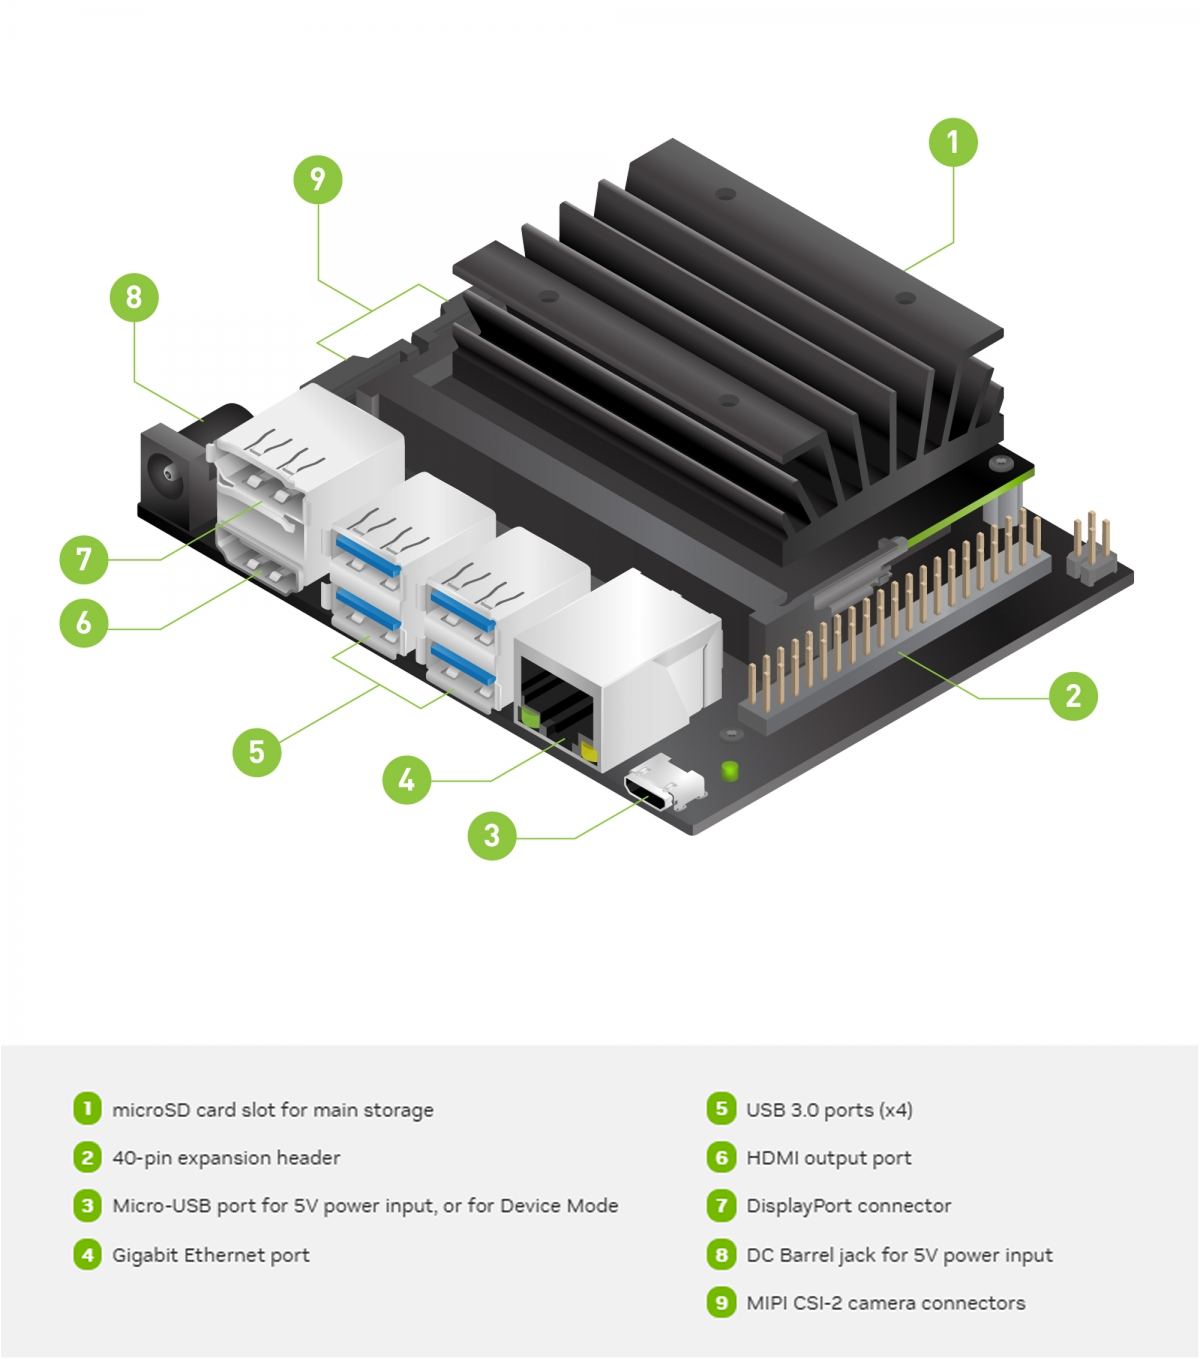
\includegraphics[width=0.6\textwidth]{figures/deployment/jetson-components.png}
\caption{Main components of the NVIDIA Jetson Nano developer kit used for edge deployment.}
\label{fig:jetson_components}
\end{figure}

The Jetson Nano runs a custom operating system image built by NVIDIA, known as Linux for Tegra (L4T), which is an Ubuntu 18.04‑based distribution specifically tailored for the Jetson hardware. This image ships with the JetPack SDK (version 4.x), providing a full development environment that includes CUDA 10, cuDNN, and TensorRT, all pre‑configured to leverage the Maxwell GPU. The kernel and device drivers are optimised for the Nano’s power management, multimedia engines, and camera interfaces, ensuring that the entire software stack—from low‑level sensor capture to GPU‑accelerated inference—can be executed without additional integration effort.

% The 128‑core Maxwell GPU delivers 472 GFLOPS of half‑precision performance, enabling real‑time inference of moderately sized neural networks.
% Combined with a quad‑core Cortex‑A57 CPU and 4 GB of fast LPDDR4 memory, the platform can execute the instrument recognition pipeline described in this thesis with low latency.
% Hardware‑accelerated H.265 encoding and decoding allow direct processing of high‑resolution video streams, while the MIPI CSI‑2 lanes and Gigabit Ethernet interface provide flexible options for camera integration and data transfer.
% The module’s 10 W maximum power draw makes it viable for continuous operation in a standalone embedded setting without active cooling.

\subsection{Limitations of the Jetson Nano}
While the Jetson Nano offers a compelling balance of performance, power efficiency and affordability. It comes with several
limitations that must be considered when deploying the models and developing the monitoring interface. Table \ref{tab:jetson_nano_limitations} summerizes the key constraints and their implications.

\begin{table}[H]
\centering
\caption{Limitations of the Jetson Nano and their practical implications.}
\label{tab:jetson_nano_limitations}
\begin{tabular}{@{}p{5cm}p{10cm}@{}}
\toprule
\textbf{Limitation} & \textbf{Implication} \\
\midrule
Limited storage and RAM & The deployed model and monitoring platform must be lightweight in both disk footprint and memory consumption; large models or extensive logging can exhaust storage, while memory‑intensive operations risk out‑of‑memory errors or performance degradation from swapping. \\
\midrule
Modest computing power & Models need to be compact and inference‑optimised (e.g., TensorRT engines, quantised formats) to achieve real‑time performance without overwhelming the processor. \\
\midrule
No active cooling (Heatsink Only) & Continuous temperature monitoring is essential to prevent throttling or hardware damage, especially under sustained GPU load in enclosures with limited airflow. \\
\midrule
Uncommon Architecture (aarch64) & Many third‑party libraries either lack official ARM64 builds or are distributed only as unofficial, potentially outdated, community‑maintained alternatives, complicating dependency management and reducing reliability. \\
\bottomrule
\end{tabular}
\end{table}

\section{Models Deployment on the Jetson Nano}






% ── General Conclusion ──────────────────────────────────────
% ============================================================
% Chapter 6: Conclusion
% ============================================================
\chapter{Conclusion}
\label{ch:conclusion}

\section{Summary of Contributions}
\label{sec:summary}

Recapitulate the main contributions of this thesis. Restate the research
problem, the methodology used, and the key findings.

\section{Answers to Research Questions}
\label{sec:answers}

Provide concise answers to each research question posed in
Chapter~\ref{ch:introduction}, based on the evidence presented in the thesis.

\section{Future Work}
\label{sec:future-work}

Suggest directions for future research that build on the work presented
in this thesis. Identify open problems, potential extensions, and
alternative approaches that could be explored.

\section{Final Remarks}
\label{sec:final-remarks}

Offer concluding thoughts on the significance of the research and its
place within the broader academic and practical landscape.


% ── Bibliography ────────────────────────────────────────────
\bibliographystyle{apalike}
\bibliography{references,zotero_refs}

% ── Appendices ──────────────────────────────────────────────
\appendix
% ============================================================
% Appendices
% ============================================================

\chapter{Additional Tables}
\label{app:tables}

Supplementary tables that support the main text but are too detailed to
include in the body of the thesis.

\begin{table}[htbp]
    \centering
    \caption{Supplementary data}
    \label{tab:supplementary}
    \begin{tabular}{lccc}
        \toprule
        \textbf{Item} & \textbf{Value A} & \textbf{Value B} & \textbf{Value C} \\
        \midrule
        Row 1 & --- & --- & --- \\
        Row 2 & --- & --- & --- \\
        \bottomrule
    \end{tabular}
\end{table}

\chapter{Additional Figures}
\label{app:figures}

Supplementary figures that provide additional context or detail.

\chapter{Code Listings}
\label{app:code}

Key source code implementations referenced in the methodology.

\begin{lstlisting}[language=Python, caption={Example implementation}, label={lst:example}]
def example_function(x):
    return x * 2
\end{lstlisting}

\chapter{Detailed Proofs}
\label{app:proofs}

If your thesis contains mathematical derivations that are too lengthy for
the main text, include the full proofs here.


\end{document}
